\chapter{Searching for Supersymmetry in the Single Lepton Channel at CMS}
\label{sec:susysearch}
\section{Introduction}
The \PW polarisation measurement, as well as being an interesting analysis in
its own right, also finds application to searches for \acl{NP}. The first of
these, comes from a more complete understanding of the \MET distribution in
\Wjets events - an important background to many \ac{SUSY} searches. The second,
is that the polarisation of the \PW coupled with the methods described in the
previous chapter provides a means to discrimate \ac{SUSY} events from \ac{SM}
backgrounds. This will be further explored in the following section.

\section{Separating \ac{SUSY} and \ac{SM} Events}
\label{sec:susy_sm}
In the context of \Rparity conserving \ac{SUSY}, a typical event with a charged
lepton in the final state is expected to contain 3 invisible particles: two
\acp{LSP} and a neutrino. As a result, the total \MET in an event will often be
larger than the transverse momentum of the charged lepton and relatively
uncorrelated with it in terms of direction. In contrast, the large boost and
polarisation of a typical \PW decay lead to a more even balance between the \MET
and the transverse momentum of the charged lepton, as well as greater
correlation of their directions. These two consideration can be applied to both
\Wjets and \ttbar events - the two dominant backgrounds to a single lepton
\ac{SUSY} search.

In order to make use of the \PW polarisation effects described, this analysis
makes use of the \LP variable as described in Section~\ref{sec:wpol_lp}. For
events containing a charged lepton and \MET originating from a \PW decay with
large transverse momentum, the alignment of the charged lepton and neutrino
gives an \LP distribution confined to the range $[0,1]$. In contrast, for
\ac{SUSY} events the \MET component is larger than the lepton momentum and thus
the \PtWv is likely to point in the direction of the \METv. Since the direction
of the charged lepton momentum and \METv will be mostly uncorrelated, \LP is
likely to tend to small values. Rewriting,
\begin{equation}
\LP = \frac{\Ptl}{\PtW}\cos\left(\PtWv, \Ptlv\right)
\end{equation}
it can be seen that in cases where the angle between the \METv and \Ptlv is more
than 90\degrees, \LP will become negative.

A second important difference between \ac{SUSY} and \ac{SM} events is related to
the overall energy scale of the events. As discussed in Chapter~\ref{sec:susy},
\ac{SUSY} decays are expected to begin with initial states much heavier than in
\ac{SM} events. To provide some measure of this energy scale without biasing the
polarisation, the variable \STlep is constructed as follows,
\begin{equation}
\STlep = \Ptl + \MET
\end{equation}
where it should be noted that \STlep is a scalar quantity. For \PW decays,
$\STlep \approx \PtW$. Since the energy scale of \ac{SUSY} is unknown, \STlep is
used to define search regions. This allows the search to be optimised without
introducing a strong dependence on the energy scale. For the purposes of this
analysis, 4 \STlep bins are employed. These are: $150 < \STlep < 250$, $250 <
\STlep < 350$, $350 < \STlep < 450$ and $\STlep > \unit{450}{\GeV}$. The lowest
region, $\STlep_{150}$ is taken to be at too low an energy scale to contain
\ac{SUSY} processes not excluded by previous searches. It is used as a sideband
to validate the analysis method.

\section{Analysis Method}
The \LP distributions for \ac{SM} backgrounds and two benchmark \ac{SUSY} models
are shown in Figure~\ref{fig:susy_lp}. The benchmark points LM1 and LM6
correspond to the \ac{CMSSM} points $(\Mzero, \Mhalf) = (60, 250)$ and $(85,
400)$ respectively, with $\tanbeta =10$ and $\Azero = 0$. Firstly it can be seen
that the heuristic discussion of the \LP shape given in
Section~\ref{sec:susy_sm} is confirmed by the simulation - with \ac{SM} events
at $\LP > 0$ and \ac{SUSY} events clustering around $\LP \sim 0$.
\begin{figure}
\centering
\subfloat[\Pe $250 < \STlep < 350$]{\label{fig:susy_lp_el_st250}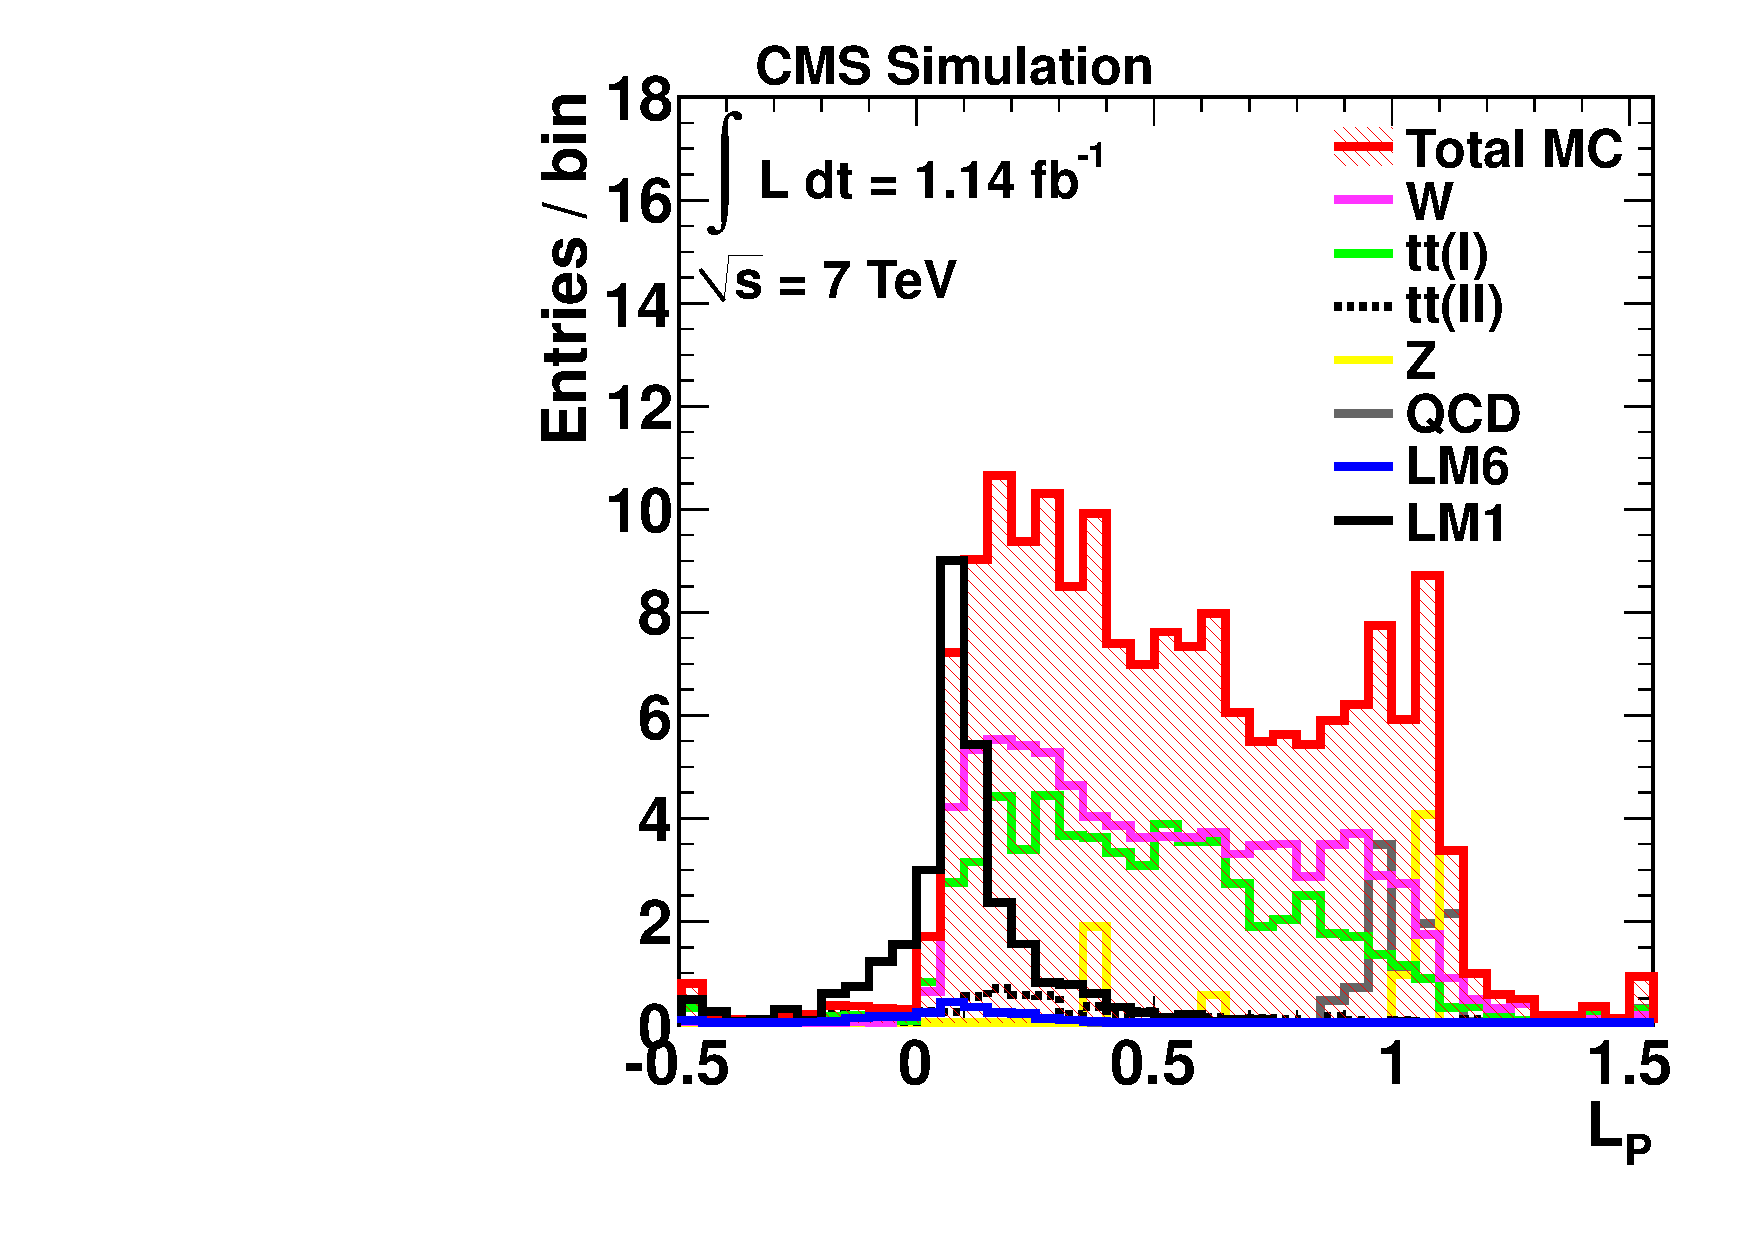
\includegraphics[width=0.3\textwidth]{fig/LP250_MCandSignal_El.pdf}}\quad
\subfloat[\Pe $350 < \STlep < 450$]{\label{fig:susy_lp_el_st350}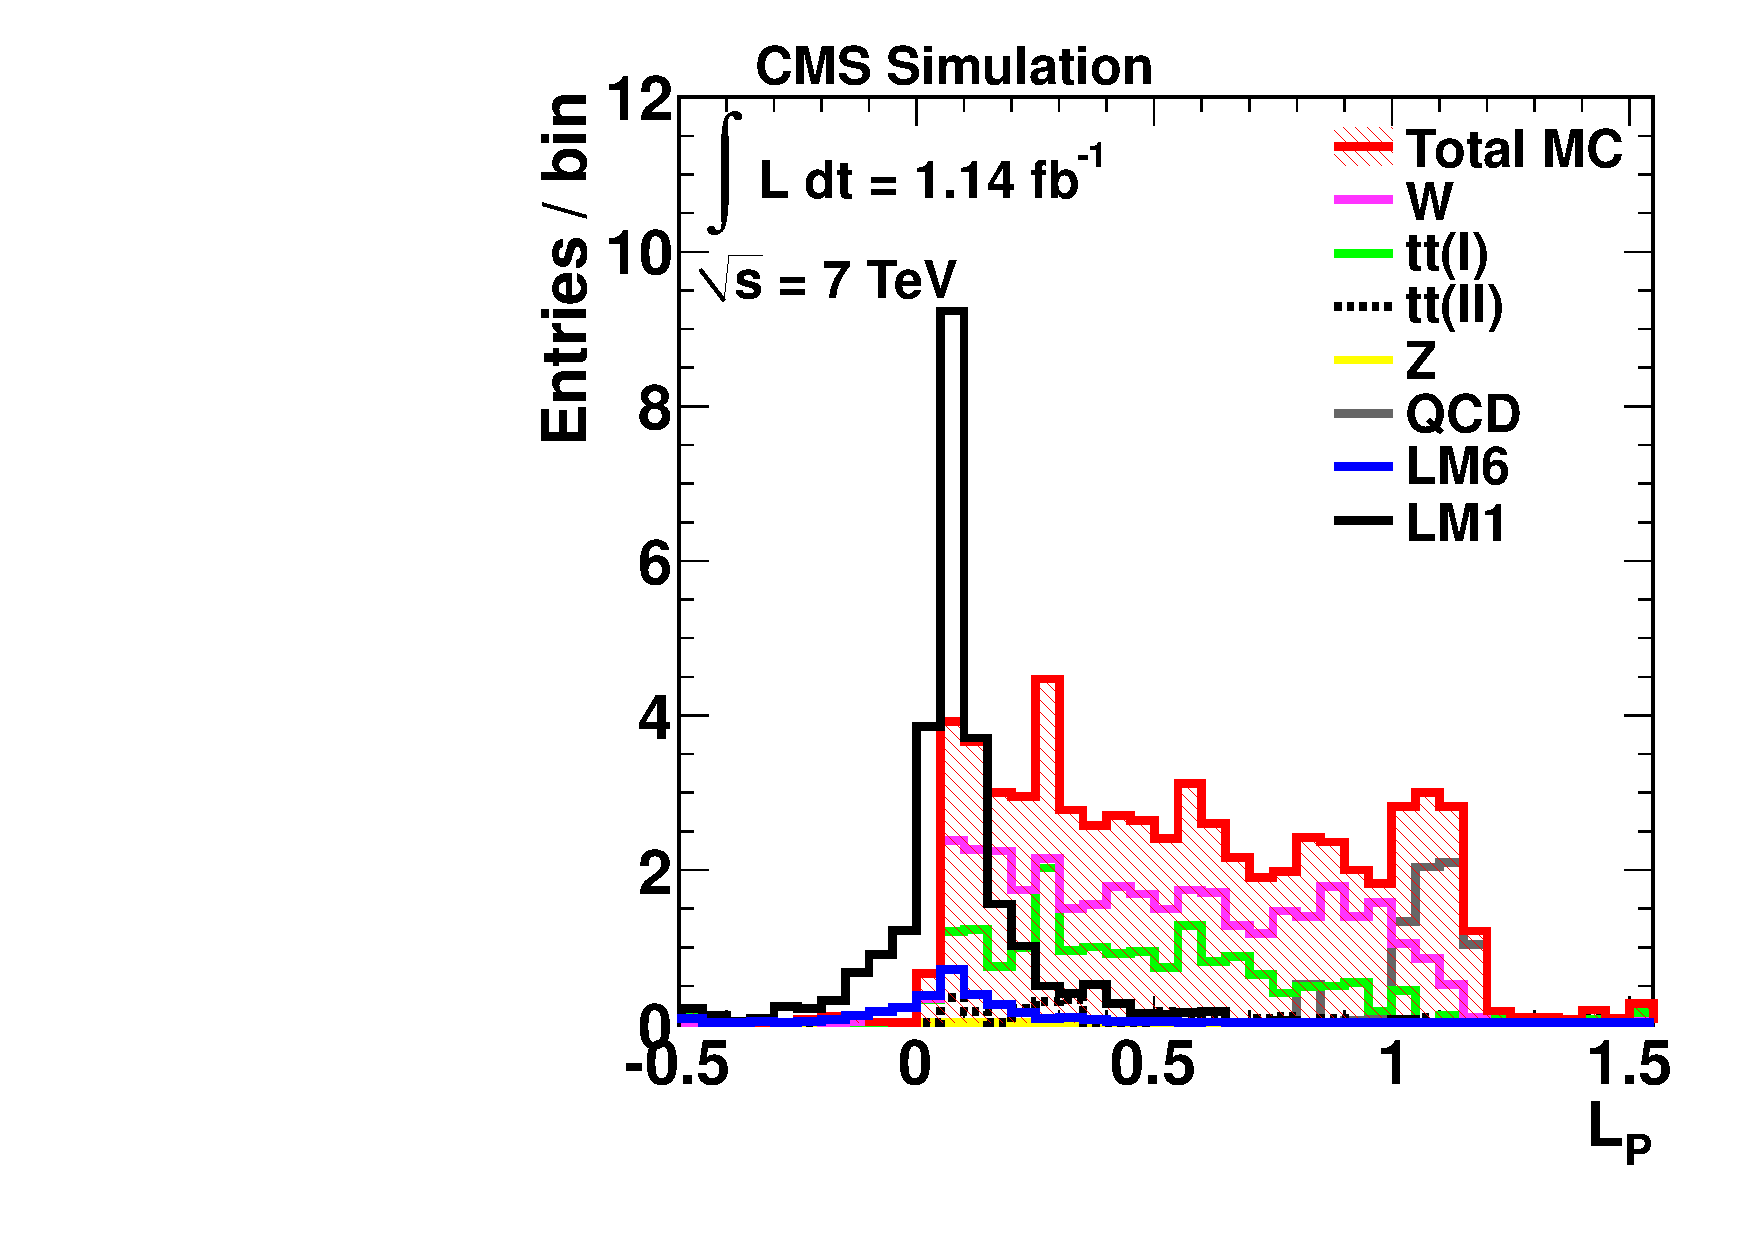
\includegraphics[width=0.3\textwidth]{fig/LP350_MCandSignal_El.pdf}}\quad
\subfloat[\Pe $\STlep > 450$]{\label{fig:susy_lp_el_st450}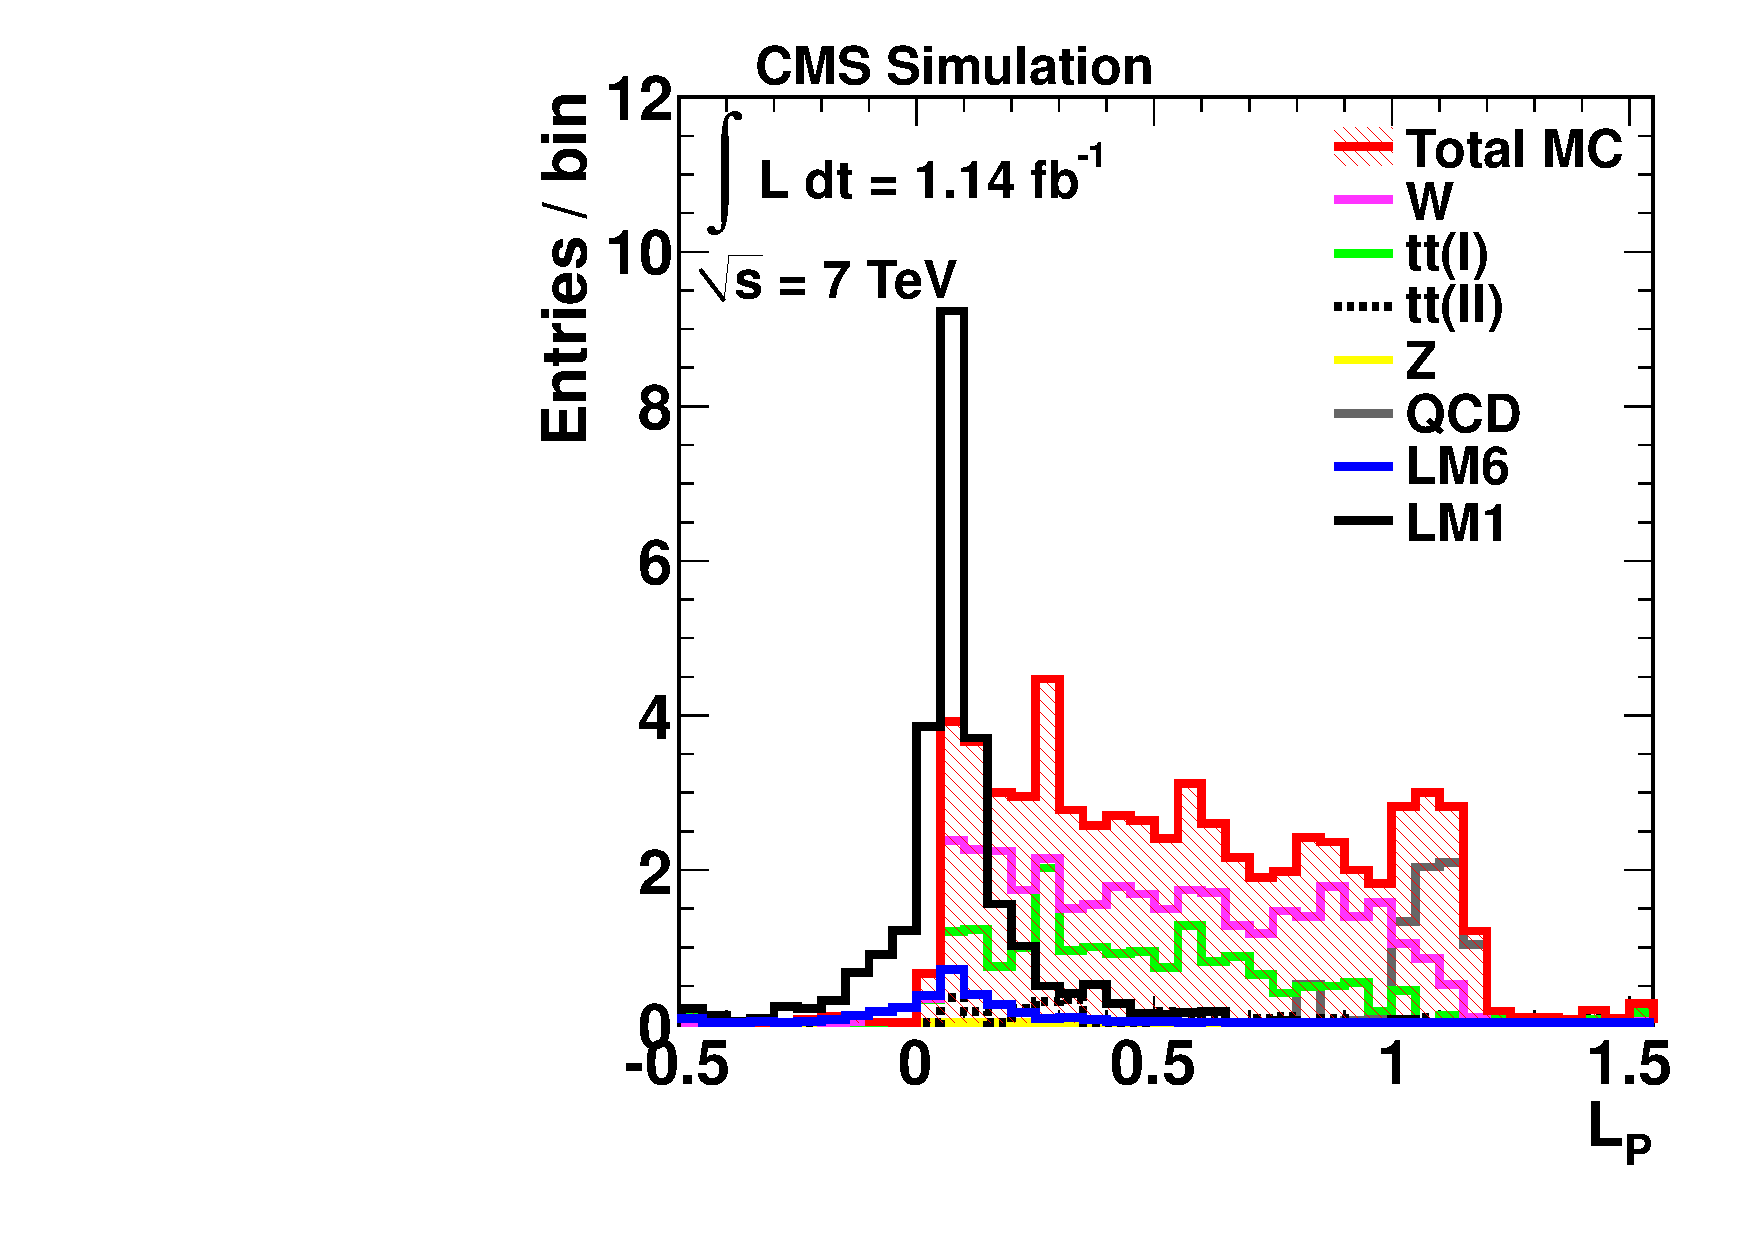
\includegraphics[width=0.3\textwidth]{fig/LP350_MCandSignal_El.pdf}}\\
\subfloat[\Pmu $250 < \STlep < 350$]{\label{fig:susy_lp_mu_st250}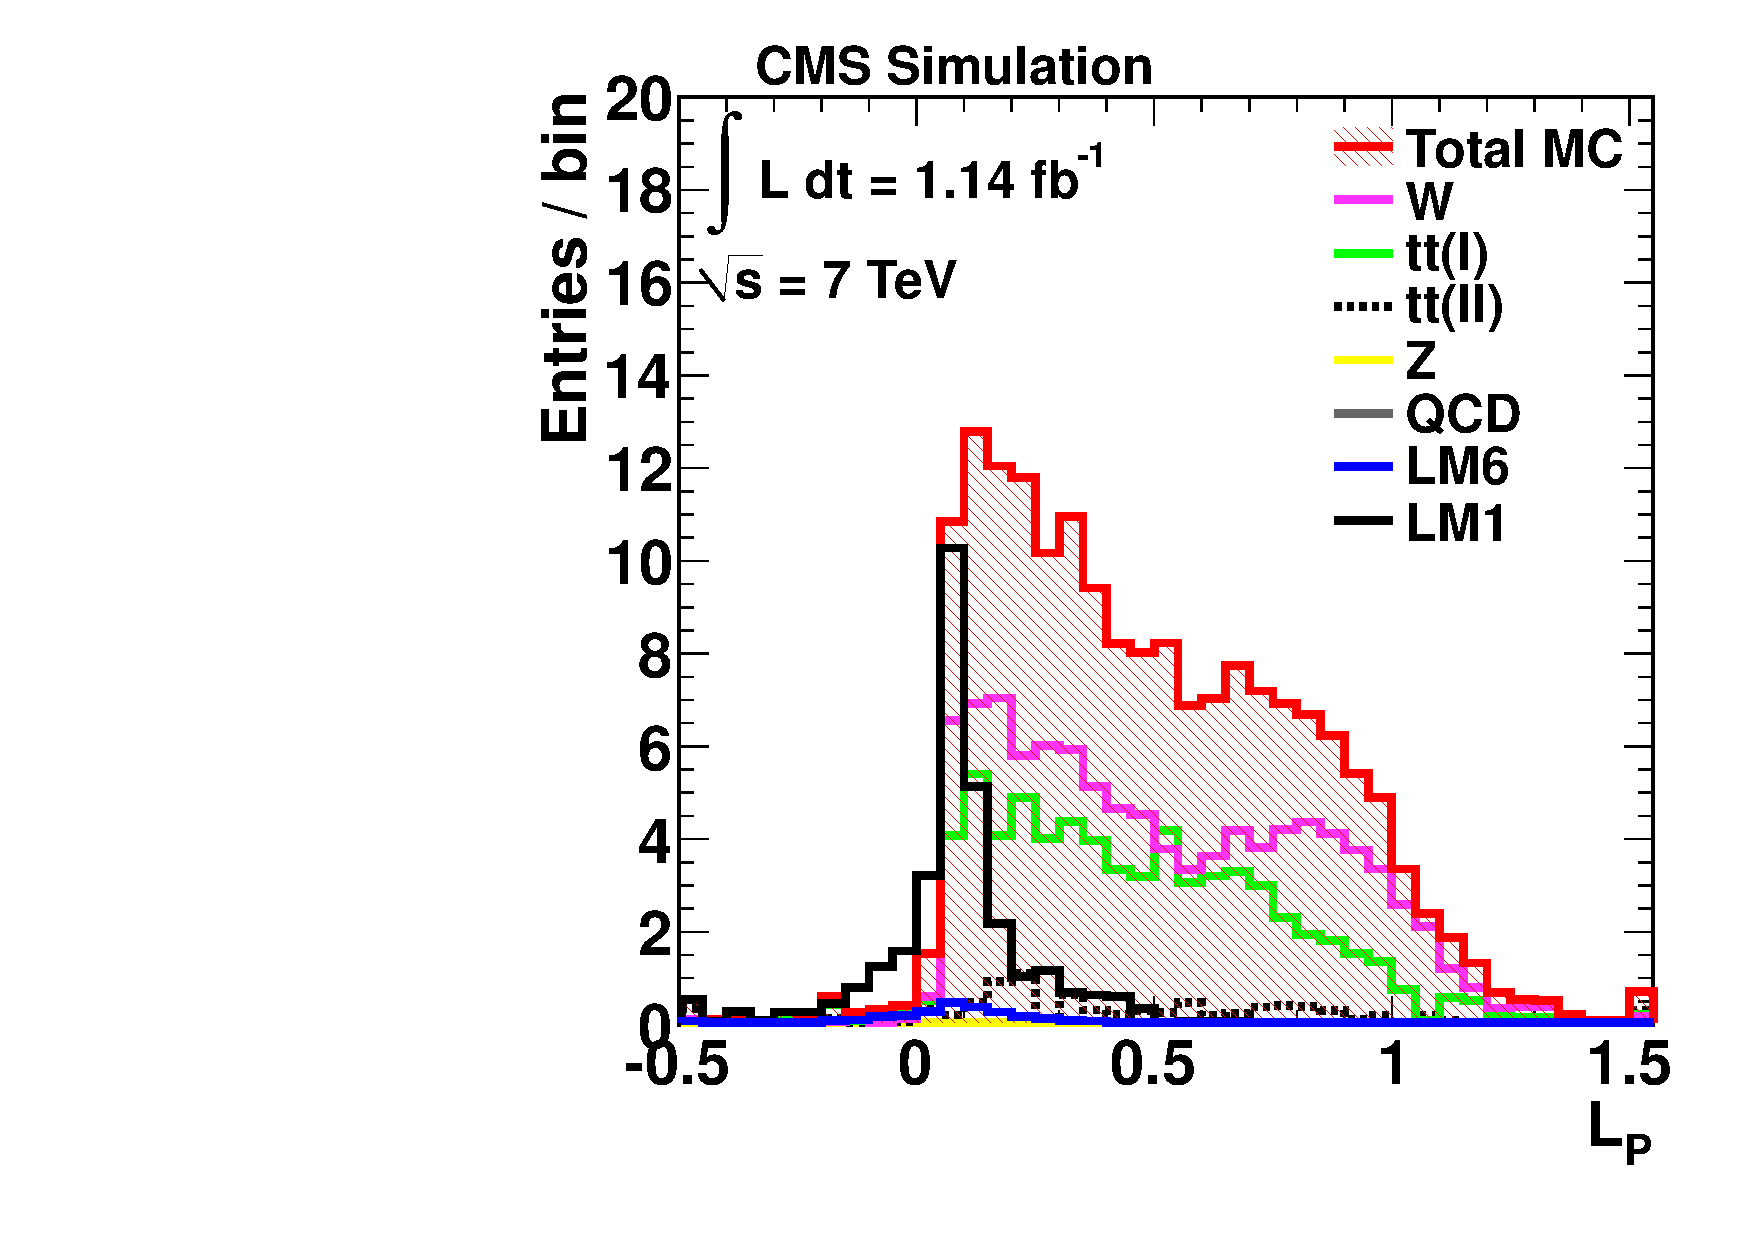
\includegraphics[width=0.3\textwidth]{fig/LP250_MCandSignal_Mu.pdf}}\quad
\subfloat[\Pmu $350 < \STlep < 450$]{\label{fig:susy_lp_mu_st350}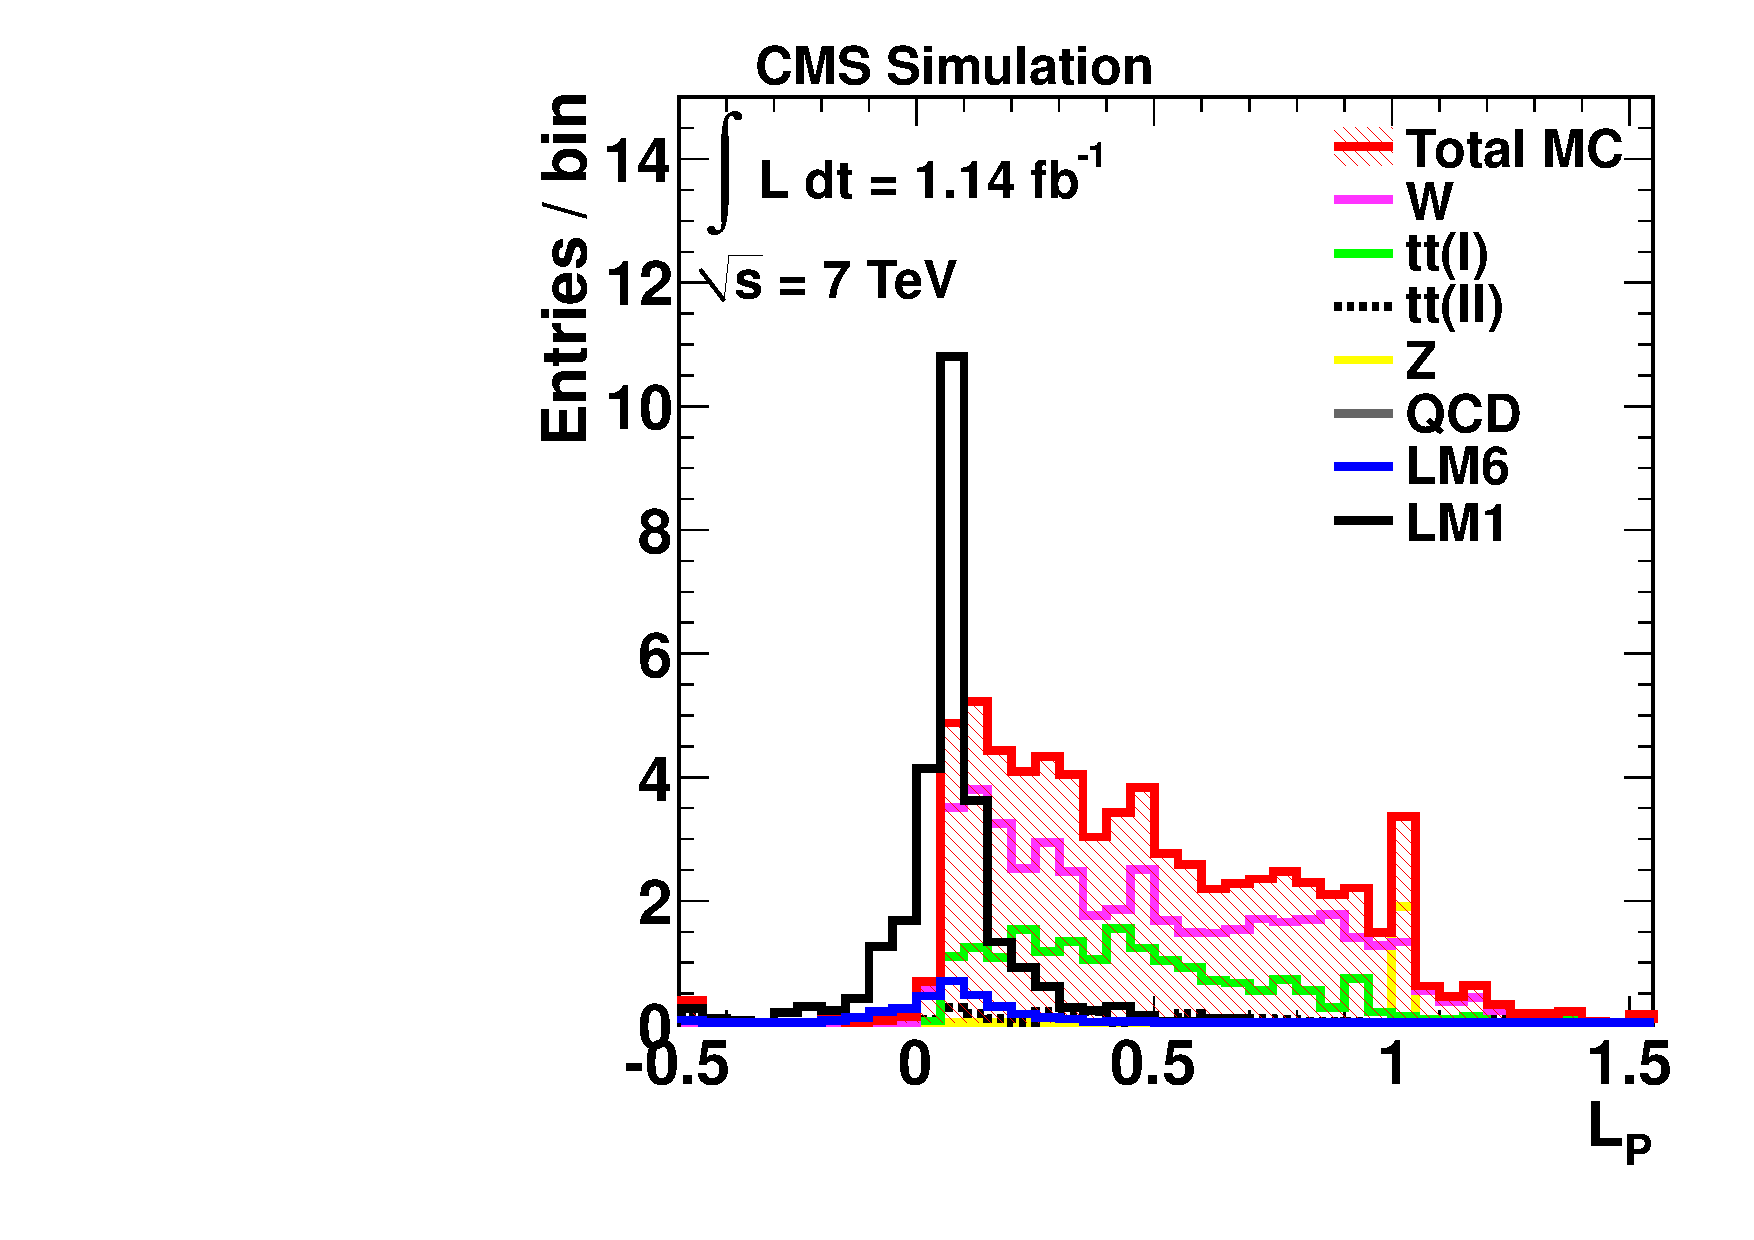
\includegraphics[width=0.3\textwidth]{fig/LP350_MCandSignal_Mu.pdf}}\quad
\subfloat[\Pmu $\STlep > 450$]{\label{fig:susy_lp_mu_st450}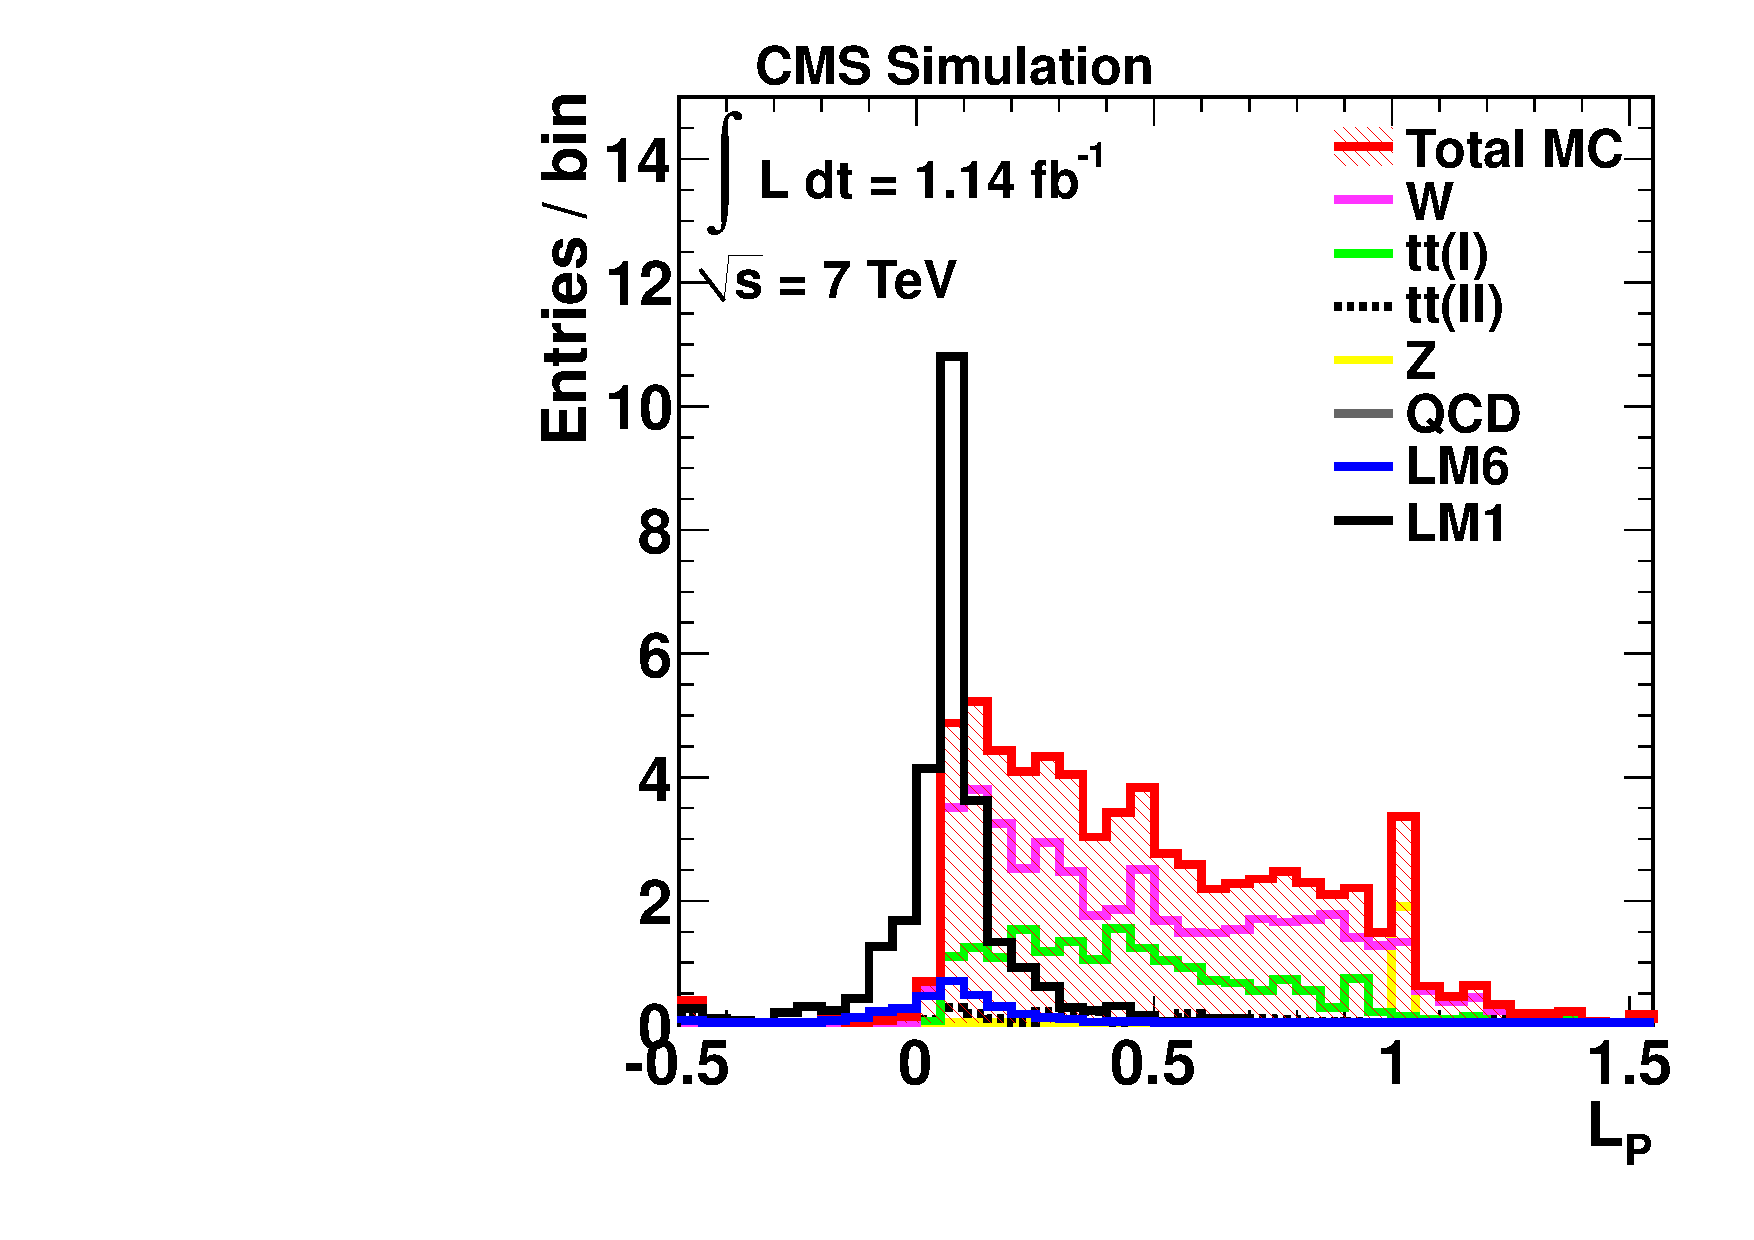
\includegraphics[width=0.3\textwidth]{fig/LP350_MCandSignal_Mu.pdf}}
\caption{Distributions showing the \LP variable for each \STlep bin}
\label{fig:susy_lp}
\end{figure}

In order to make use of the discrimination power afforded by the \LP shape, a
signal and control region are defined. The signal region is defined such that an
enriched sample of \ac{SUSY} events is obtained without being highly model
dependent. It should be stressed that the intent is not to eliminate the
background altogether in this region. The control region likewise must select a
sample of \ac{SM} background events with sufficient statistics whilst guarding
against excessive signal contamination from \ac{SUSY} models. By studying the
\LP distribution across the \ac{CMSSM} parameter space, \LPsignal for the signal
region and \LPcontrol for the control region were found to be suitable choices.

To predict the \ac{SM} background contamination in the \LPsignal region, a
translation factor, \RCS is calculated in simulation. This is defined as
\begin{equation}
\RCS = \frac{N^{\textrm{MC}}(\LPsignal)}{N^{\textrm{MC}}(\LPcontrol)}
\label{eqn:susysearch_RCS}
\end{equation}
where $N^{\textrm{MC}}(\LPsignal)$ and $N^{\textrm{MC}}(\LPcontrol)$ represent
the population, as calculated in simulation of \ac{SM} events in the signal and
control regions respectively. Once calculated, \RCS may be used along with a
measurement of the control region in data to predict the \ac{SM} background
contribution present in the signal region,
\begin{equation}
N^{\textrm{data}}(\LPsignal) = \RCS N^{\textrm{data}}(\LPcontrol)
\end{equation}
Whilst in principle it is possible to perform a more, or even completely,
data-driven prediction by performing a template fit to the \LP shape in the
control region and extrapolating into the signal region, this strategy was
explored for some time and found to be frustrated by inadequate statistics, even
at relatively large integrated luminosities.

The advantage of the translation factor \RCS is that by taking the ratio from
simulation, there is significant cancellation of many systematic uncertainties,
including in particular the jet energy scale that proved to be significant for
the \PW polarisation analysis (see Section~\ref{sec:wpol_syst_jec}). Since these
uncertainties do not cancel completely, they will be full evaluated in
Section~\ref{sec:susy_systematics} and are included in the statistical treatment
described in Chapter~\ref{sec:interpretation}.

One last point concerning \RCS is that, so that the prediction is not dominated
by uncertainties stemming from limited statistics in the control region, a value
of $\RCS << 1$ is preferable. As we will see, relatively small values of \RCS
are obtained using the definitions given above.

\section{Object Definitions}
The basic object selection requirements were defined to be consistent between
several complementary leptonic \ac{SUSY} searches at \ac{CMS}. They are
described and motivated further in~\cite{susy_selection_an}.

\subsection{Jets and Missing Energy}
Jets and missing energy quantities are taken from the particle flow algorithm,
as described in Section~\ref{sec:reco_pf}. In addition, jets are required to
pass the ``LOOSE'' selection criteria, namely
\begin{itemize}
\item At least two particles - at least one of them charged - in the jet.
\item Fraction of jet energy carried by neutral hadrons less than 99\%.
\item Charged and neutral electromagnetic fractions both less than 99\%.
\end{itemize}
All jets are required to have a transverse momentum, $\Pt > \unit{40}{\GeV}$ and
are required to be within the fiducial region of the tracker, $|\eta| <
2.4$. The total hadronic transverse energy, \HT is calculated from jets passing
this selection.

\subsection{Muons}
Muon reconstruction is described in Section~\ref{sec:reco_muons}. Global muons
are selected with a number of additional quality requirements. These are similar
to thoseused in the \PW polarisation analysis (see Section~\ref{sec:wpol_muons})
with certain adjustements made to ensure consistency with other analyses or
adapt to the different analysis requirements.
\begin{itemize}
\item A normalized $\chi^2 < 10$ on the global muon fit
\item More than 10 hits in the tracker (including at least 1 pixel hit) and
  $\geq 2$ matching segments in the muon chambers.
\item A transverse distance to the nominal interaction point, $d_0 <
  \unit{200}{\micro\metre}$ and longitudinal distance to the primary vertex $d_z
  < \unit{1}{\centi\metre}$
\item The uncertainty on the muon transverse momentum $\sigma(\Pt)/\Pt^2 <
  \unit{0.001}{\reciprocal\GeV}$
\item Each global muon must also qualify as a tracker muon.
\item A combined relative isolation (see Eqn~\ref{eqn:wpol_mu_comb_iso}) $\CombIso < 0.1$.
\end{itemize}

\textbf{Tight} muons are defined by the requirements given above. \textbf{Loose}
muons use an identical selection but with the \CombIso cut loosened to 0.15.

\subsection{Electrons}
\textbf{Tight} electrons are reconstructed as described in
Section~\ref{sec:reco_electrons} using the 80\% efficiency working point but
with impact parameter requirements identical to those used for the
muons. \textbf{Loose} electrons use the 95\% efficiency working point with the
impact parameter criteria loosened as for the muon case.

\subsection{Resolving Ambiguities}
Since the leptons used in this analysis use the traditional reconstruction
methods at \ac{CMS} while jets and \METv are taken from the \ac{PF} algorithm,
ambiguities can exist. In order to avoid double counting, these ambiguities are
resolved by several cleaning steps.

To remove jets dominated by a lepton, any jet found within a cone of 0.1 (0.3)
of a selected muon (electron) is removed from consideration. In addition, muons
within a cone of 0.3 of any jet are rejected.

A second step corrects the \METv for differences between \ac{PF} and global muon
reconstruction. Each global muon is matched to a corresponding \ac{PF} muon
within a cone of $\DeltaR < 0.1$. The absolute relative difference between the
transverse momenta is then calculated. For cases where no match is found or this
difference is $> 20\%$, the event is rejected. For cases where the difference is
smaller than 20\%, the \METv receives a vectorial correction.

\section{Analysis Selection}
Selection begins with a set of event cleaning cuts common to many analyses at
\ac{CMS}. These address known detector and reconstruction problems as well as
supressing machine backgrounds. They are fully detailed in~\cite{susy_selection_an}.

Lepton selection requires exactly one \textbf{Tight} electron or muon. To remove
dilepton events and minimise overlap with searches in multilepton final states,
events containing a second \textbf{Loose} lepton are vetoed.

After the initial lepton selection cuts, events can enter two independent
samples. The first is a control sample, inverting the jet multiplicity cut to
obtain a sample known to be overwhelmingly dominated by \ac{SM} backgrounds. To
compensate, this sample is selected with a slightly relaxed \HT cut. The second
sample is then used for the final analysis. A jet multiplicity cut, $\Njets \geq
3$ is applied as well as an \HT cut.

The data-driven control sample was used to test the analysis techniques before
applying them to the search dataset. During this time, the search dataset was
not studied (or ``blinded'') to avoid changes in the analysis procedure that
might bias the result. Once the analysis method was fully refined, the search
sample was ``unblinded'' and major changes to the analysis were no longer
allowed.

Due to the unavailability of suitable efficient and unbiased triggers, the
control sample was considered only for the muon channel. For the electron
channel, validation work was performed instead in the $150 < \STlep <
\unit{250}{\GeV}$ bin. Trigger thresholds in the control sample necessitated
increasing the transverse momentum cut on the muon to \unit{35}{\GeV}.

The full sequence of selection requirements is shown in
Table~\ref{tbl:susy_cutflow}. The corresponding event yields, as measured in
simulation are shown in Tables~\ref{tbl:susy_mcexp_signal} and
\ref{tbl:susy_mcexp_control} for the signal and control regions respectively.

\ctable[
cap=\acs{SUSY} search selection requirements,
caption=Selection requirements for the \ac{SUSY} search in both the search
samples and the muon control sample. The lepton selection and veto requirements
are common to both samples.,
pos=h,
label=tbl:susy_cutflow
]{ll}{
}{\FL
Lepton Selection           & Exactly one \textbf{Tight} electron or muon \NN
                           & $|\eta^{\Pgm}| < 2.1$, $|\eta^{\Pe}| < 2.5$\NN
Lepton Veto                & Zero additional leptons passing \textbf{Loose} criteria\NN
                           & $P_T^{\Pgm} > \unit{15}{\GeV}$, $P_T^{\Pe} > \unit{20}{\GeV}$\NN
                           & $|\eta^{\Pgm}| < 2.5$, $|\eta^{\Pe}| < 2.5$\ML
Control Sample (\Pgm only) & $< 3$~jets \NN
                           & $P_T^{\Pgm} > \unit{35}{\GeV}$\NN
                           & $\HT > \unit{200}{\GeV}$ \ML
Analysis Sample            & $\geq 3$~jets \NN
                           & $P_T^{\Pl} > \unit{20}{\GeV}$\NN
                           & $\HT > \unit{500}{\GeV}$\LL
}
\ctable[
caption=Expected event yields in the signal region\, $\LP < 0.15$\, with
\unit{1.14}{\invfb} in the muon and electron channels.  The MC values are only
listed for illustration purposes.  The actual estimate of the number of SM
events in the signal region uses the method described in the text. The
contribution from QCD multijet production is expected to be negligible and is
thus not included in the table.,
pos=h!,
label=tbl:susy_mcexpectation_signal,
%doinside=\scriptsize
]{ccccccc}{
}{\FL
$\LP<0.15$          & \multicolumn{3}{c}{ Muons: \STlep range (GeV) } & \multicolumn{3}{c}{  Electrons: \STlep range (GeV) }\ML
Sample              & [250-350]                                         & [350-450]    & [450-$\inf$] & [250-350]   & [350-450]   & [450-$\inf$] \ML
\ttbar ($\ell$)     & 11.4$\pm$0.9                                      & 2.91$\pm$0.4 & 0.8$\pm$0.2  & 7.8$\pm$0.7 & 3.0$\pm$0.4 & 1.0$\pm$0.3\NN
\ttbar ($\ell\ell$) & 2.2$\pm$0.4                                       & 0.6$\pm$0.2  & 0.1$\pm$0.1
                    & 2.4$\pm$0.4                                       & 0.7$\pm$0.2  & 0.4$\pm$0.2\NN
W                   & 14.5$\pm$0.6                                      & 8.0$\pm$0.5  & 5.6$\pm$0.4
                    & 10.5$\pm$0.5                                      & 5.2$\pm$0.4  & 4.7$\pm$0.3\NN
Z                   & 0$\pm$1.5                                         & 0$\pm$1.5    & 0$\pm$1.5
                    & 0$\pm$1.5                                         & 0$\pm$1.5    & 0$\pm$1.5\NN
Total MC            & 28.1$\pm$1.1                                      & 11.5$\pm$0.7 & 6.5$\pm$0.4
                    & 20.8$\pm$1.0                                      & 8.8$\pm$0.6  & 6.1$\pm$0.5\NN
LM1                 & 24.2$\pm$0.9                                      & 23.1$\pm$0.9 & 16.2$\pm$0.7
                    & 22.9$\pm$0.9                                      & 20.8$\pm$0.8 & 14.7$\pm$0.7\NN
LM3                 & 24.8$\pm$0.8                                      & 16.7$\pm$0.6 & 9.7$\pm$0.5
                    & 22.8$\pm$0.7                                      & 14.8$\pm$0.6 & 9.7$\pm$0.5\NN
LM6                 & 1.9$\pm$0.0                                       & 2.5$\pm$0.1  & 5.9$\pm$0.1
                    & 1.7$\pm$0.0                                       & 2.3$\pm$0.1  & 5.3$\pm$0.1 \LL
}
\ctable[
caption=Expected event yields in the control region\, $\LP > 0.30$\, with
\unit{1.14}{\invfb} in the muon and electron channels.  The MC values are only
listed for illustration purposes.  The actual estimate of the number of SM
events in the signal region uses the method described in the text.,
pos=h!,
label=tbl:susy_mcexp_control,
%doinside=\scriptsize
]{ccccccc}{
}{\FL
$\LP>0.30$          & \multicolumn{3}{c}{  Muons: \STlep range (GeV) } & \multicolumn{3}{c}{  Electrons: \STlep range (GeV) } \ML
Sample              & [250-350]                                        & [350-450]    & [450-$\inf$] & [250-350] & [350-450] & [450-$\inf$] \ML
\ttbar ($\ell$)     & 43.4$\pm$1.7                                     & 12.3$\pm$0.9 & 2.7$\pm$0.4
                    & 42.2$\pm$1.7                                     & 11.4$\pm$0.8 & 2.9$\pm$0.4\NN
\ttbar ($\ell\ell$) & 5.2$\pm$0.6                                      & 1.6$\pm$0.3  & 0.4$\pm$0.2
                    & 2.5$\pm$0.4                                      & 1.4$\pm$0.3  & 0.3$\pm$0.1\NN
W                   & 67.1$\pm$1.3                                     & 27.5$\pm$0.8 & 15.3$\pm$0.6
                    & 57.5$\pm$1.2                                     & 24.3$\pm$0.8 & 14.7$\pm$0.6\NN
Z                   & 0$\pm$1.5                                        & 1.7$\pm$1.5  & 0$\pm$1.5
                    & 7.5$\pm$3.6                                      & 0$\pm$0      & 0$\pm$0\NN
QCD                 & 0$\pm$1.5                                        & 0$\pm$1.5    & 0$\pm$1.5
                    & 10.4$\pm$3.0                                     & 7.2$\pm$1.7  & 3.8$\pm$0.7\NN
Total MC            & 116$\pm$2                                        & 43.4$\pm$2.3 & 18.4$\pm$0.8
                    & 120$\pm$5                                        & 44.3$\pm$2.1 & 21.7$\pm$1.1\NN
LM1                 & 2.8$\pm$0.3                                      & 1.4$\pm$0.2  & 0.8$\pm$0.2
                    & 2.9$\pm$0.3                                      & 2.0$\pm$0.3  & 1.3$\pm$0.2\NN
LM3                 & 9.7$\pm$0.5                                      & 4.2$\pm$0.3  & 2.3$\pm$0.2
                    & 9.1$\pm$0.5                                      & 4.2$\pm$0.3  & 2.5$\pm$0.2\NN
LM6                 & 0.5$\pm$0.0                                      & 0.4$\pm$0.0  & 0.9$\pm$0.0
                    & 0.5$\pm$0.0                                      & 0.4 $\pm$0.0 & 0.9$\pm$0.0\LL
}

\section{Triggers and Datasets}
Due to the construction of \STlep, events may be selected with moderate \MET
(and a high \Pt lepton) or large \MET (and a modertate \Pt lepton). This
necessitates a different trigger strategy to that used in other leptonic
\ac{SUSY} searches at \ac{CMS} which typically only select high \MET events.

For the search sample, a set of single-lepton cross-triggers are used, selecting
events with a single lepton in association with a large amount of hadronic
activity, \HT. As the luminosity increased during the 2011 run, it was necessary
to introduce a third requirement: a moderate cut on the \MET. The full list of
triggers used for both lepton channels are shown in
Table~\ref{tbl:susy_triggers}

\ctable[
cap=Triggers used in the \ac{SUSY} search analysis,
caption=Triggers used in the \ac{SUSY} search analysis for muon and electron search samples and the muon control sample,
pos=h!,
label=tbl:susy_triggers,
doinside=\scriptsize
]{ll}{
}{\FL
\multicolumn{2}{c}{\textbf{Search Sample}}\ML
\Pgm & HLT\_Mu8\_HT200\_v* \NN
     & HLT\_Mu15\_HT200\_v* \NN
     & HLT\_Mu15\_HT250\_PFMHT20\_v* \ML
\Pe  & HLT\_Ele10\_CaloIdL\_CaloIsoVL\_TrkIdVL\_TrkIsoVL\_HT200\_v* \NN
     & HLT\_Ele15\_CaloIdT\_CaloIsoVL\_TrkIdT\_TrkIsoVL\_HT250\_v* \NN
     & HLT\_HT250\_Ele5\_CaloIdVL\_TrkIdVL\_CaloIsoVL\_TrkIsoVL\_PFMHT35\_v* \NN
     & HLT\_HT300\_Ele5\_CaloIdVL\_TrkIdVL\_CaloIsoVL\_TrkIsoVL\_PFMHT40\_v* \ML
\multicolumn{2}{c}{\textbf{Control sample}}\ML
\Pgm & HLT\_Mu20\_v*, HLT\_IsoMu17\_v*\NN
     & HLT\_Mu30\_v*, HLT\_IsoMu24\_v*\LL
}

All signal and background Monte Carlo samples are from the Summer11 \ac{CMS}
\unit{7}{\TeV} production using \ac{CMSSW} 42. All processes are simulated using
the Madgraph matrix element generator, with the exception of the \ac{QCD} and
\ac{SUSY} signal samples which use \ac{PYTHIA} 6. All datasets, with the
exception of the \ac{SUSY} signal scan used to derive the limit use the full
detector simulation. The \ac{SUSY} signal scan uses the \ac{FASTSIM} simplified
simulation package to reduce processing time. All samples contain data-like
pile-up conditions, with a reweighting procedure used througout to reflect the
exact vertex multiplicity distribution in the data.

In addition to the standard \Wjets sample, an enriched sample with a
generator-level $\HT > \unit{300}{\GeV}$ cut. This increases the available
statistics, minimising the statistical error on \RCS.

\section{Control Region}
In order to test that the simulation of electroweak background processes can be
relied upon for the calculation of the translation factor \RCS, the procedure is
first performed in the control sample. With the jet multiplicity cut inverted,
supersymmetry signals should be highly diluted in this sample. It is expected
therefore that the background prediction in the signal region should agree well
with the observed signal yield. Furthermore, the level of agreement between data
and simulation is also important in establishing the method.

A summary of the yields in the \LPcontrol and \LPsignal regions in the $<3$~jet
control sample is given in Table~\ref{tbl:susy_control_yields}. Shown are the
yields per subprocess from simulation - used to calculate the factor \RCS, the
yields in data and the resulting background prediction. Comparing the background
prediction, it is seen to agree within errors with the observe number of events
in the signal region. The uncertainties stem from the limited data statistics of
the control region and the limited Monte Carlo statistics used in the
calculation of \RCS.

\ctable[
caption=SUSY Control Yields,
pos=h!,
label=tbl:susy_control_yields,
%doinside=\scriptsize
]{ccccccc}{
}{\FL
 & \multicolumn{3}{c}{Control Region: \LPcontrol} & \multicolumn{3}{c}{Signal Region: \LPsignal} \ML
Sample      & [250-350]    & [350-450]    & [450-$\inf$] & [250-350]             & [350-450]            & [450-$\inf$]\ML
\ttbar      & 50.1$\pm$1.8 & 7.8$\pm$0.7  & 2.8$\pm$0.4  & 10.5$\pm$0.8          & 2.8$\pm$0.4          & 0.7$\pm$0.2 \NN
W           & 959$\pm$24   & 162$\pm$9.7  & 46.2$\pm$5.2 & 83.7$\pm$7.0          & 22.8$\pm$3.7         & 12.3$\pm$2.8 \NN
Z           & 45.3$\pm$9.2 & 4.7$\pm$2.9  & 3.9$\pm$2.8  & 1.8$\pm$1.8           & 0$\pm$1.8            & 0$\pm$1.8 \NN
QCD         & 2.7$\pm$1.7  & 0.8$\pm$0.8  & 0$\pm$0.8    & 0$\pm$1.4             & 0$\pm$1.3            & 0$\pm$1.3 \NN
Total MC    & 1054$\pm$26  & 174$\pm$10.2 & 52.9$\pm$5.9 & 96$\pm$7.3            & 25.6$\pm$3.7         & 13$\pm$2.8 \NN
data        & 1051         & 179          & 52           & 92                    & 24                   & 11 \NN
SM Estimate &              &              &              & 95.8$\pm$10.2$\pm$7.6 & 26.3$\pm$5.5$\pm$4.1 & 12.8$\pm$4.0$\pm$3.0\NN
LM6         & 0.3$\pm$0.0  & 0.2$\pm$0.0  & 0.4$\pm$0.0  & 1.0$\pm$0.0           & 1.0$\pm$0.0          & 2.4$\pm$0.1 \LL
}


Comparisons of the variables \STlep, \MT and \Ptmu between data and simulation
are shown in Figure~\ref{fig:susy_mucontrol_kin}. A similar comparison is shown
for the \LP variable in bins of \STlep in
Figure~\ref{fig:susy_mucontrol_lp}. These distributions are those used to derive
the numbers shown in Table~\ref{tbl:susy_control_yields}. The data is seen to be
adequately described by the simulation.
\begin{figure}
\centering
\subfloat[\STlep]{\label{fig:susy_mucontrol_st}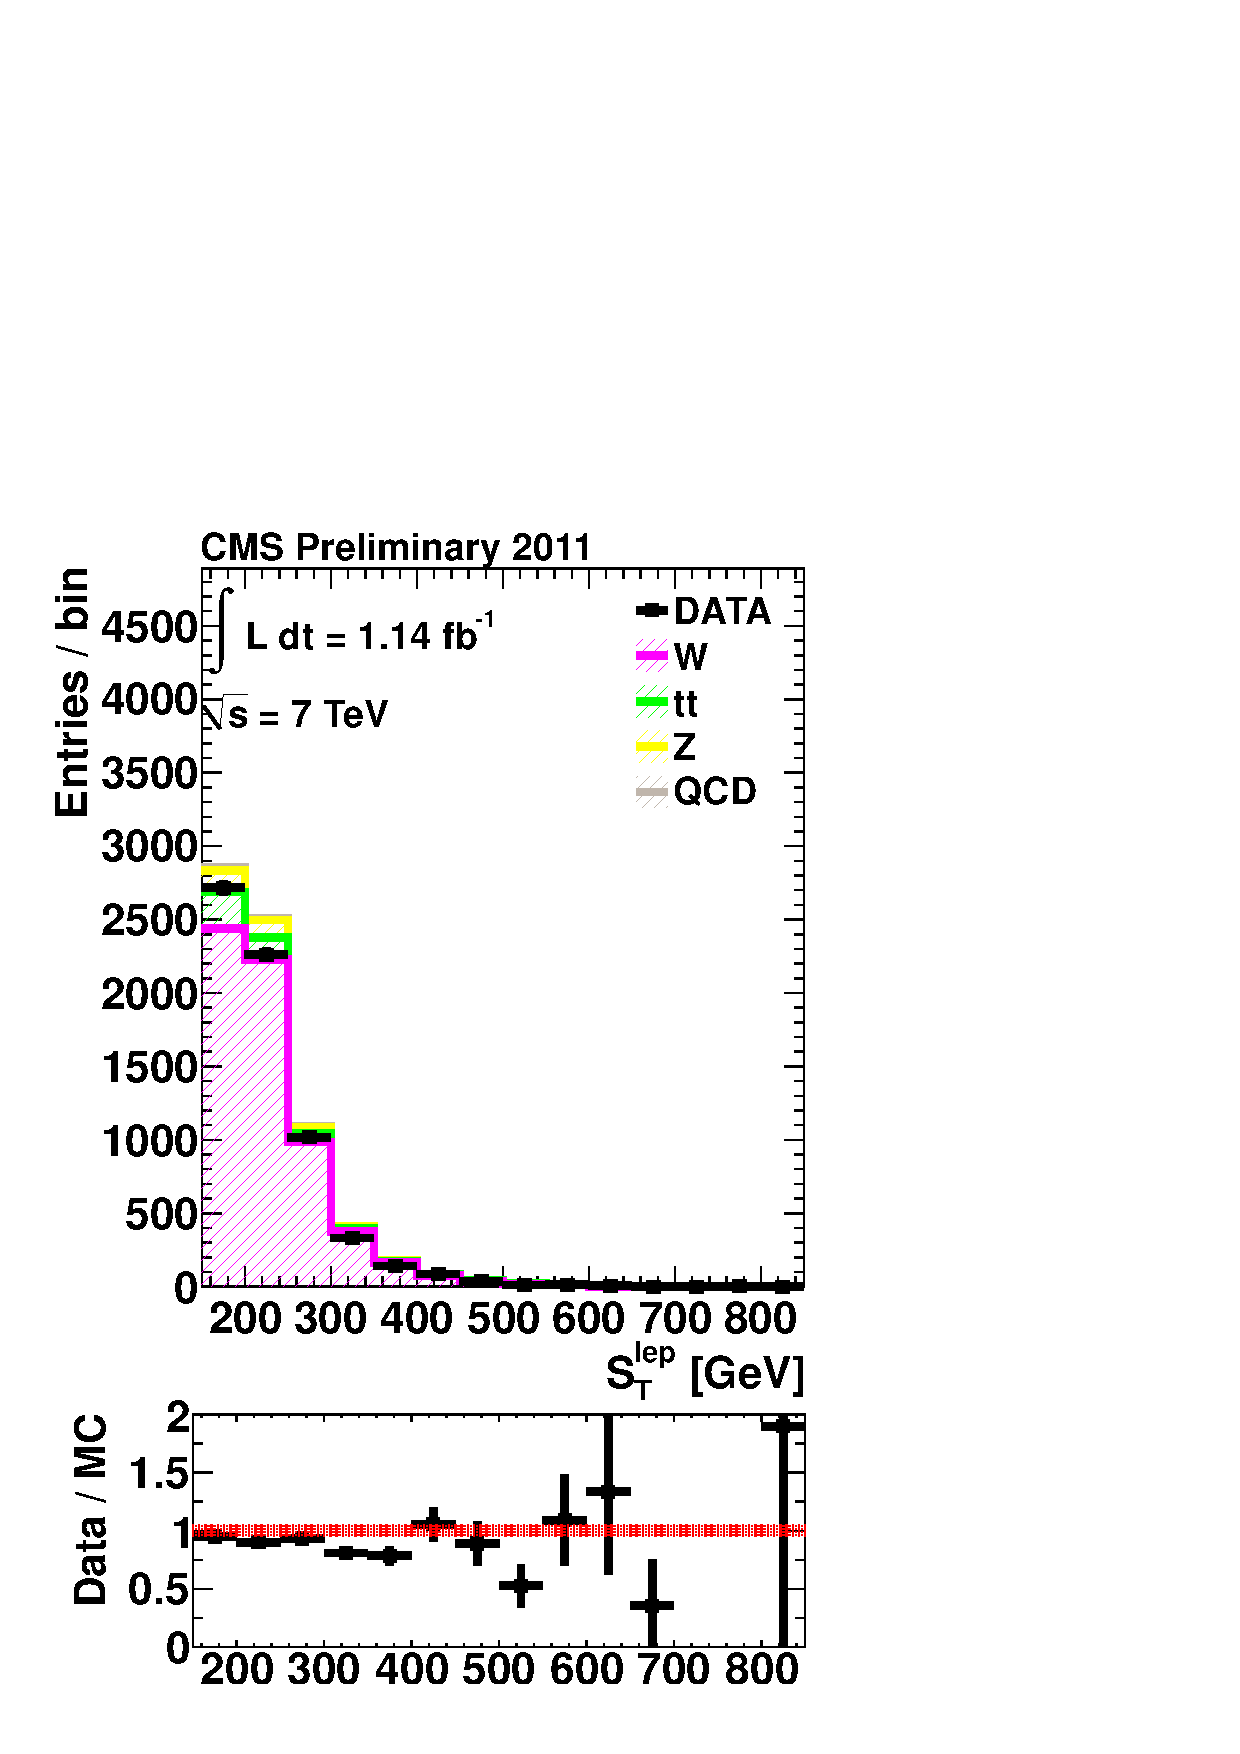
\includegraphics[width=0.3\textwidth]{fig/MuControl_ST150toInf}}\quad
\subfloat[\MT]{\label{fig:susy_mucontrol_mt}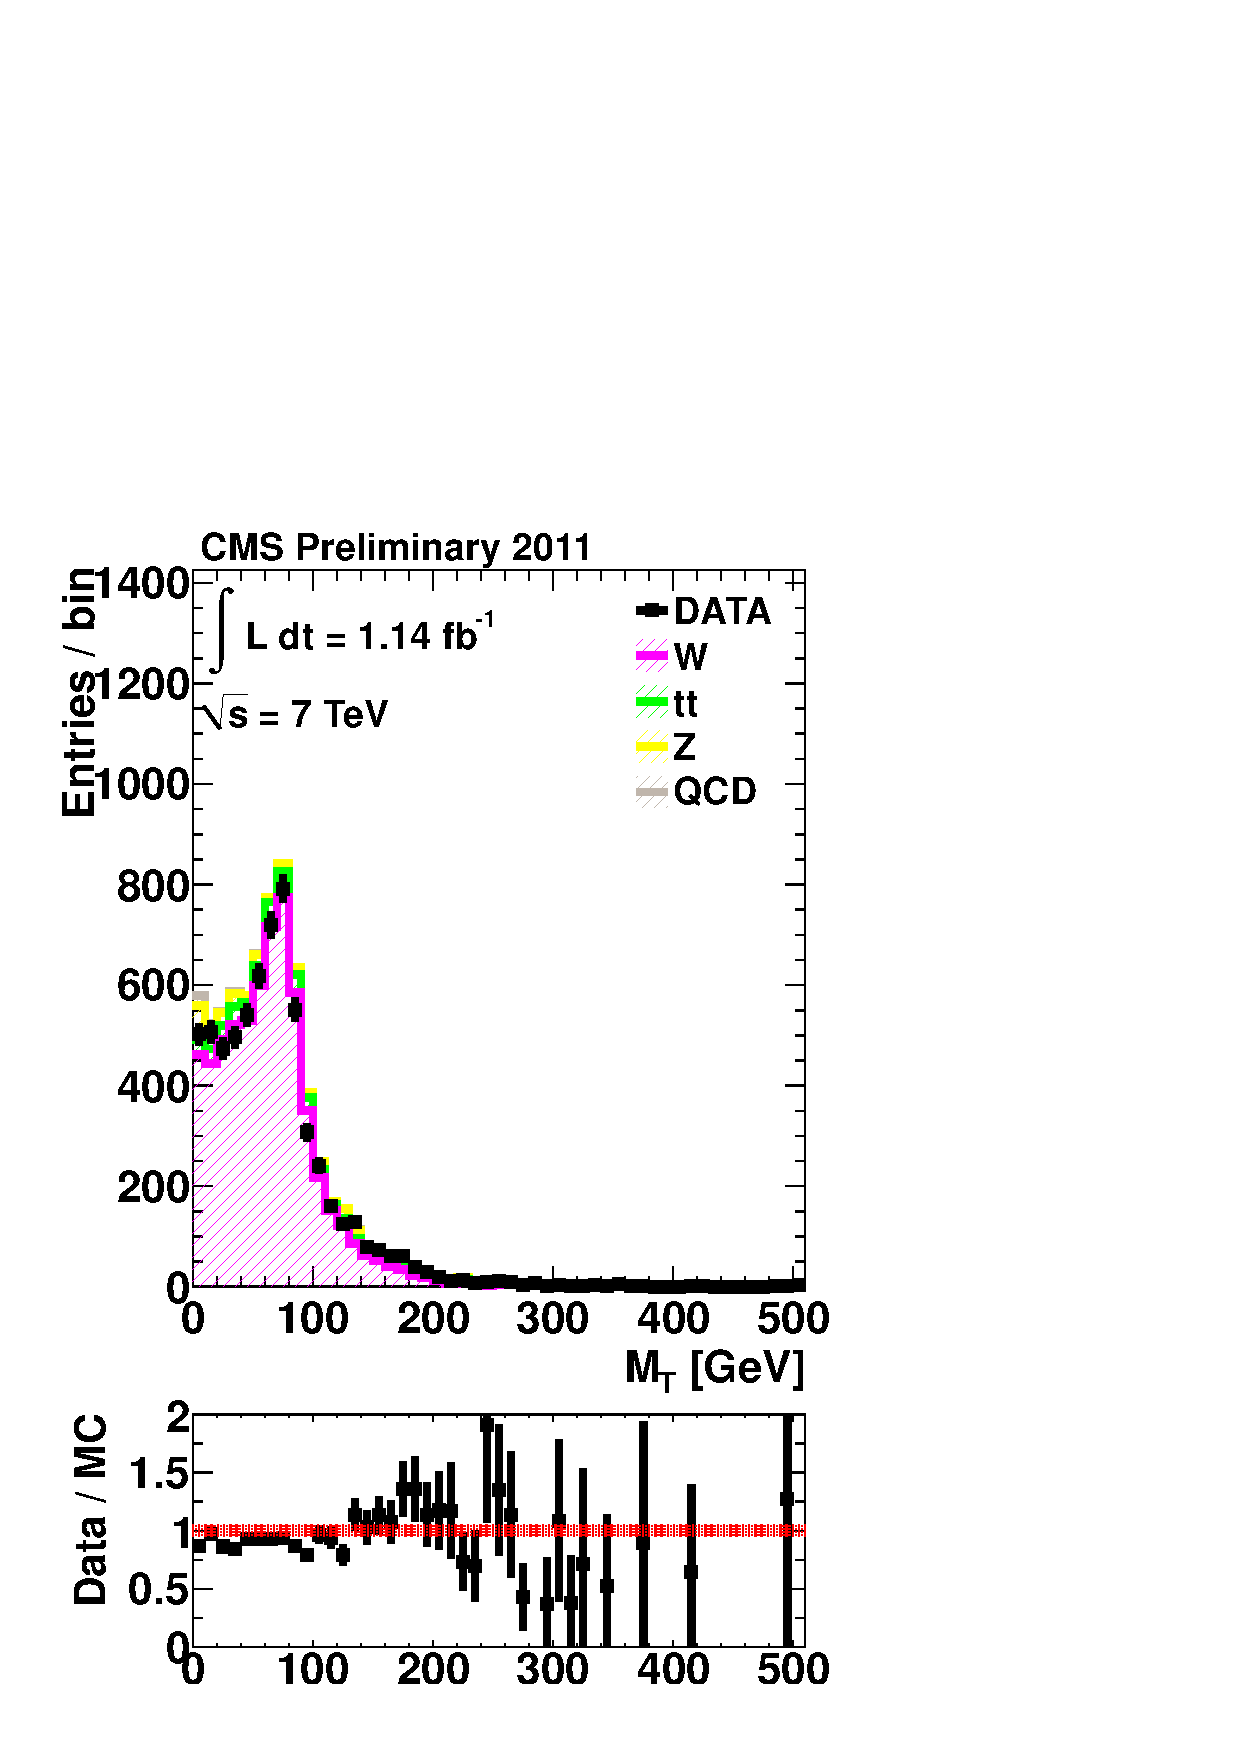
\includegraphics[width=0.3\textwidth]{fig/MuControl_MT150toInf}}\quad
\subfloat[\Ptmu]{\label{fig:susy_mucontrol_pt}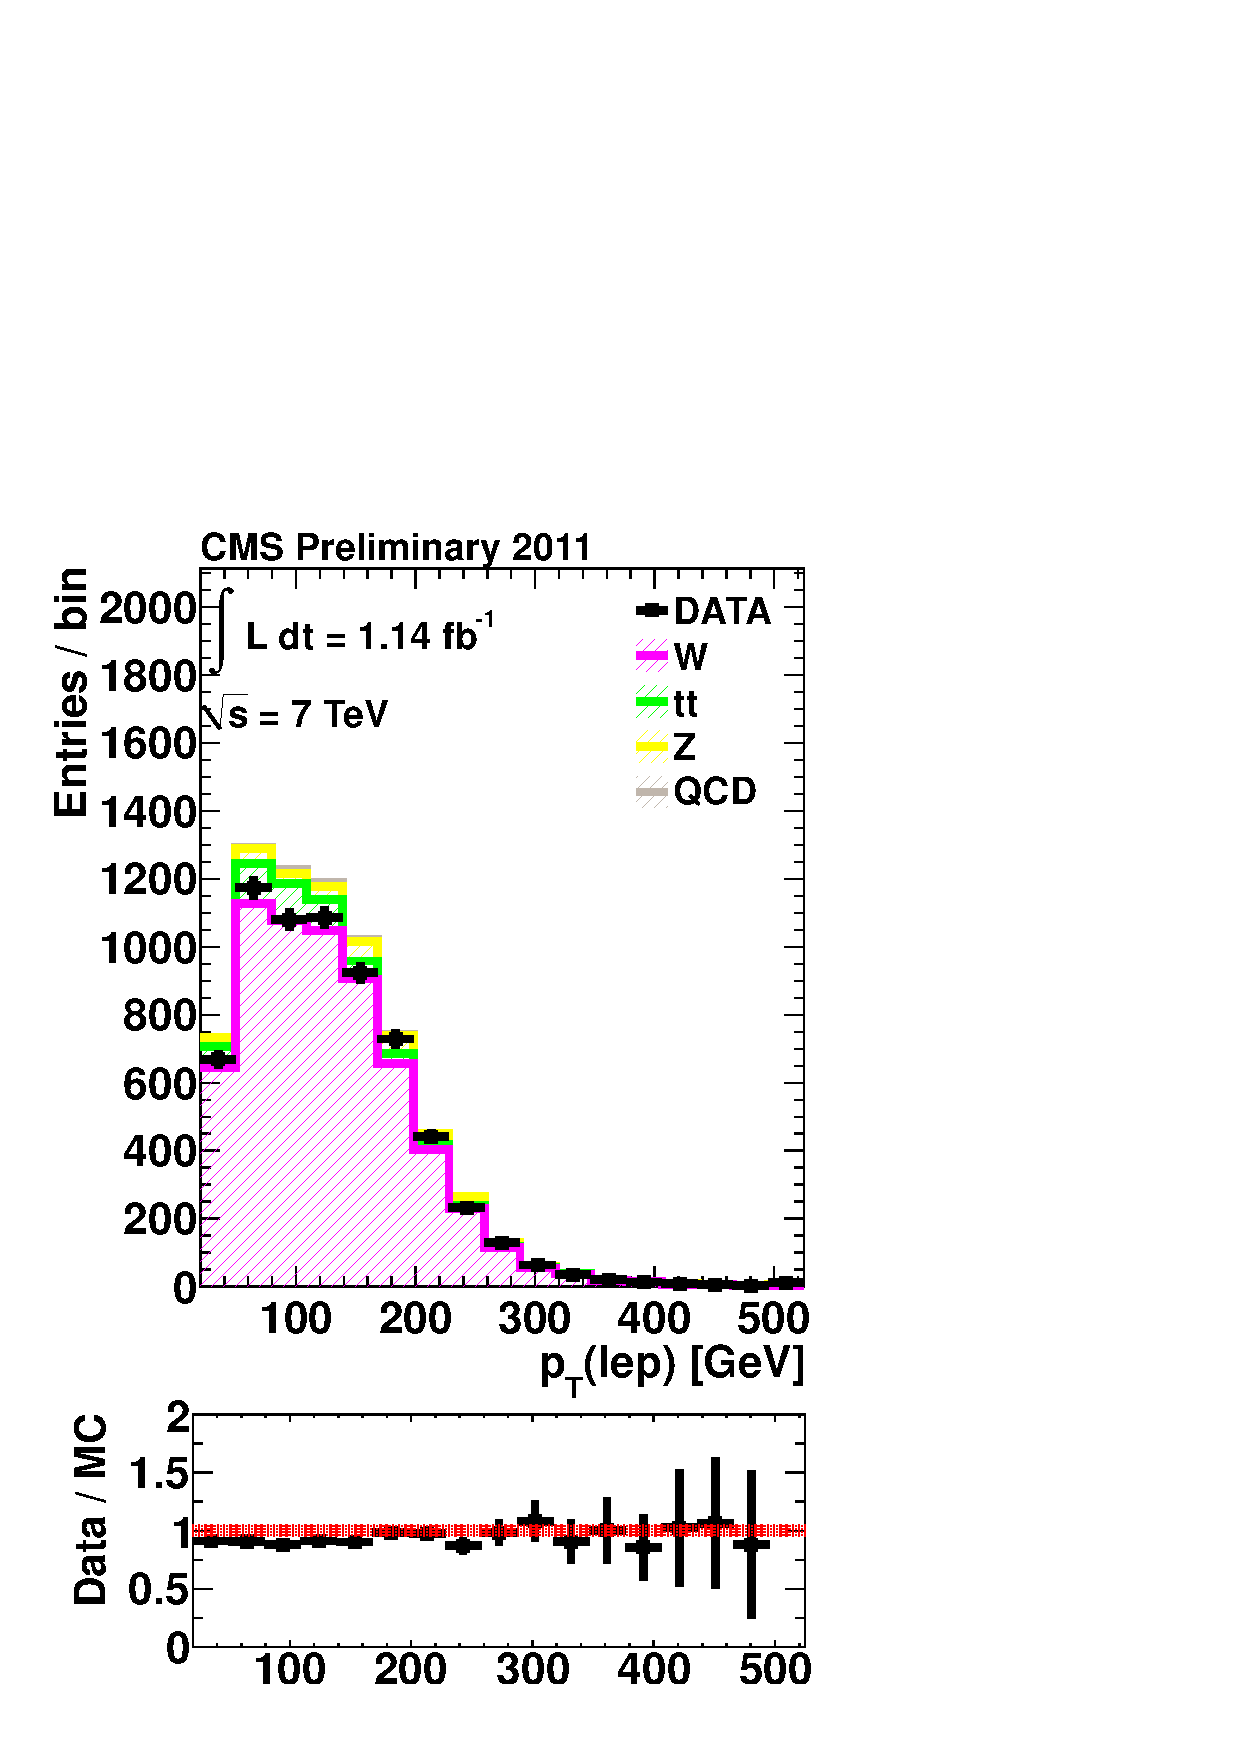
\includegraphics[width=0.3\textwidth]{fig/MuControl_MuPt150toInf}}
\caption[]{Distributions of several kinematic variables as measured in the muon control sample}
\label{fig:susy_mucontrol_kin}
\end{figure}

\begin{figure}
\centering
\subfloat[$250 < \STlep < 350$]{\label{fig:susy_mucontrol_lp250}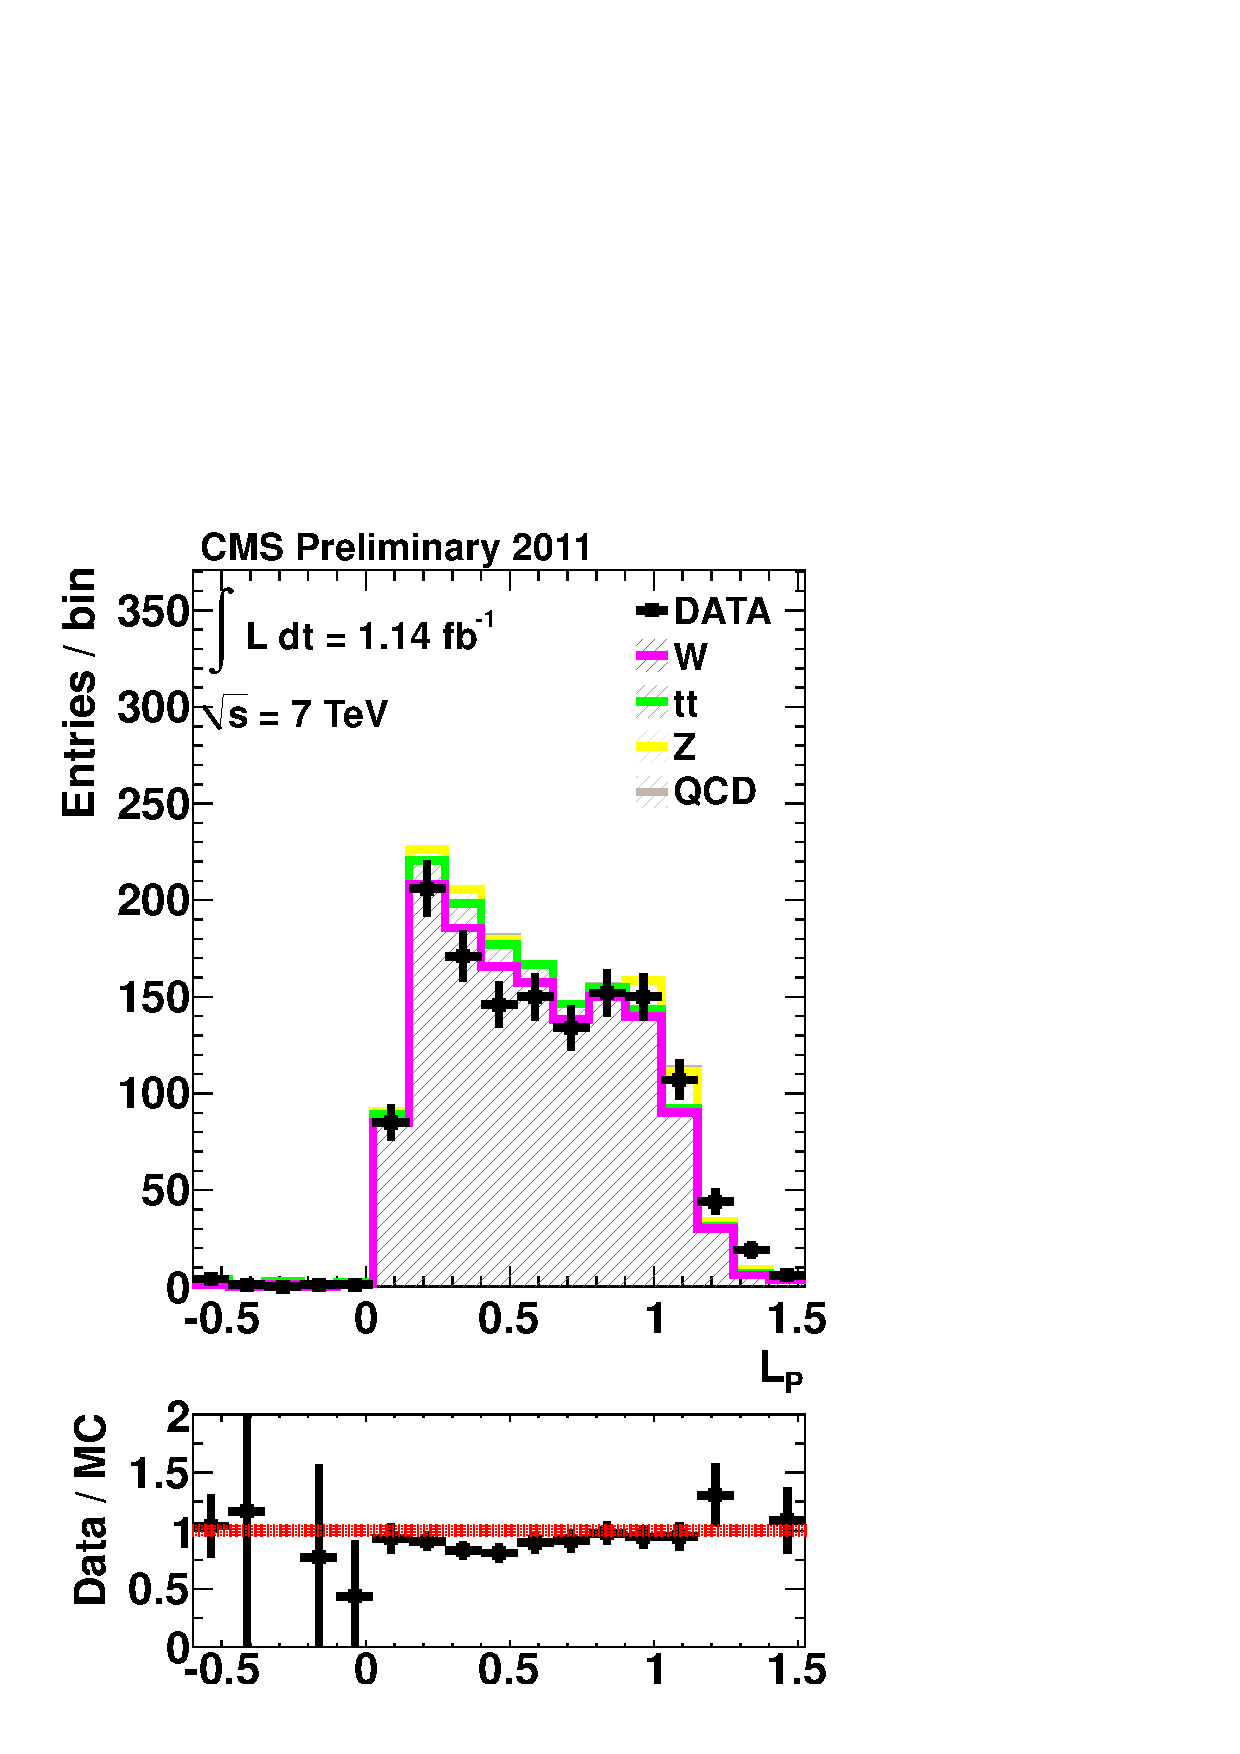
\includegraphics[width=0.3\textwidth]{fig/MuControl_LP250}}\quad
\subfloat[$250 < \STlep < 450$]{\label{fig:susy_mucontrol_lp350}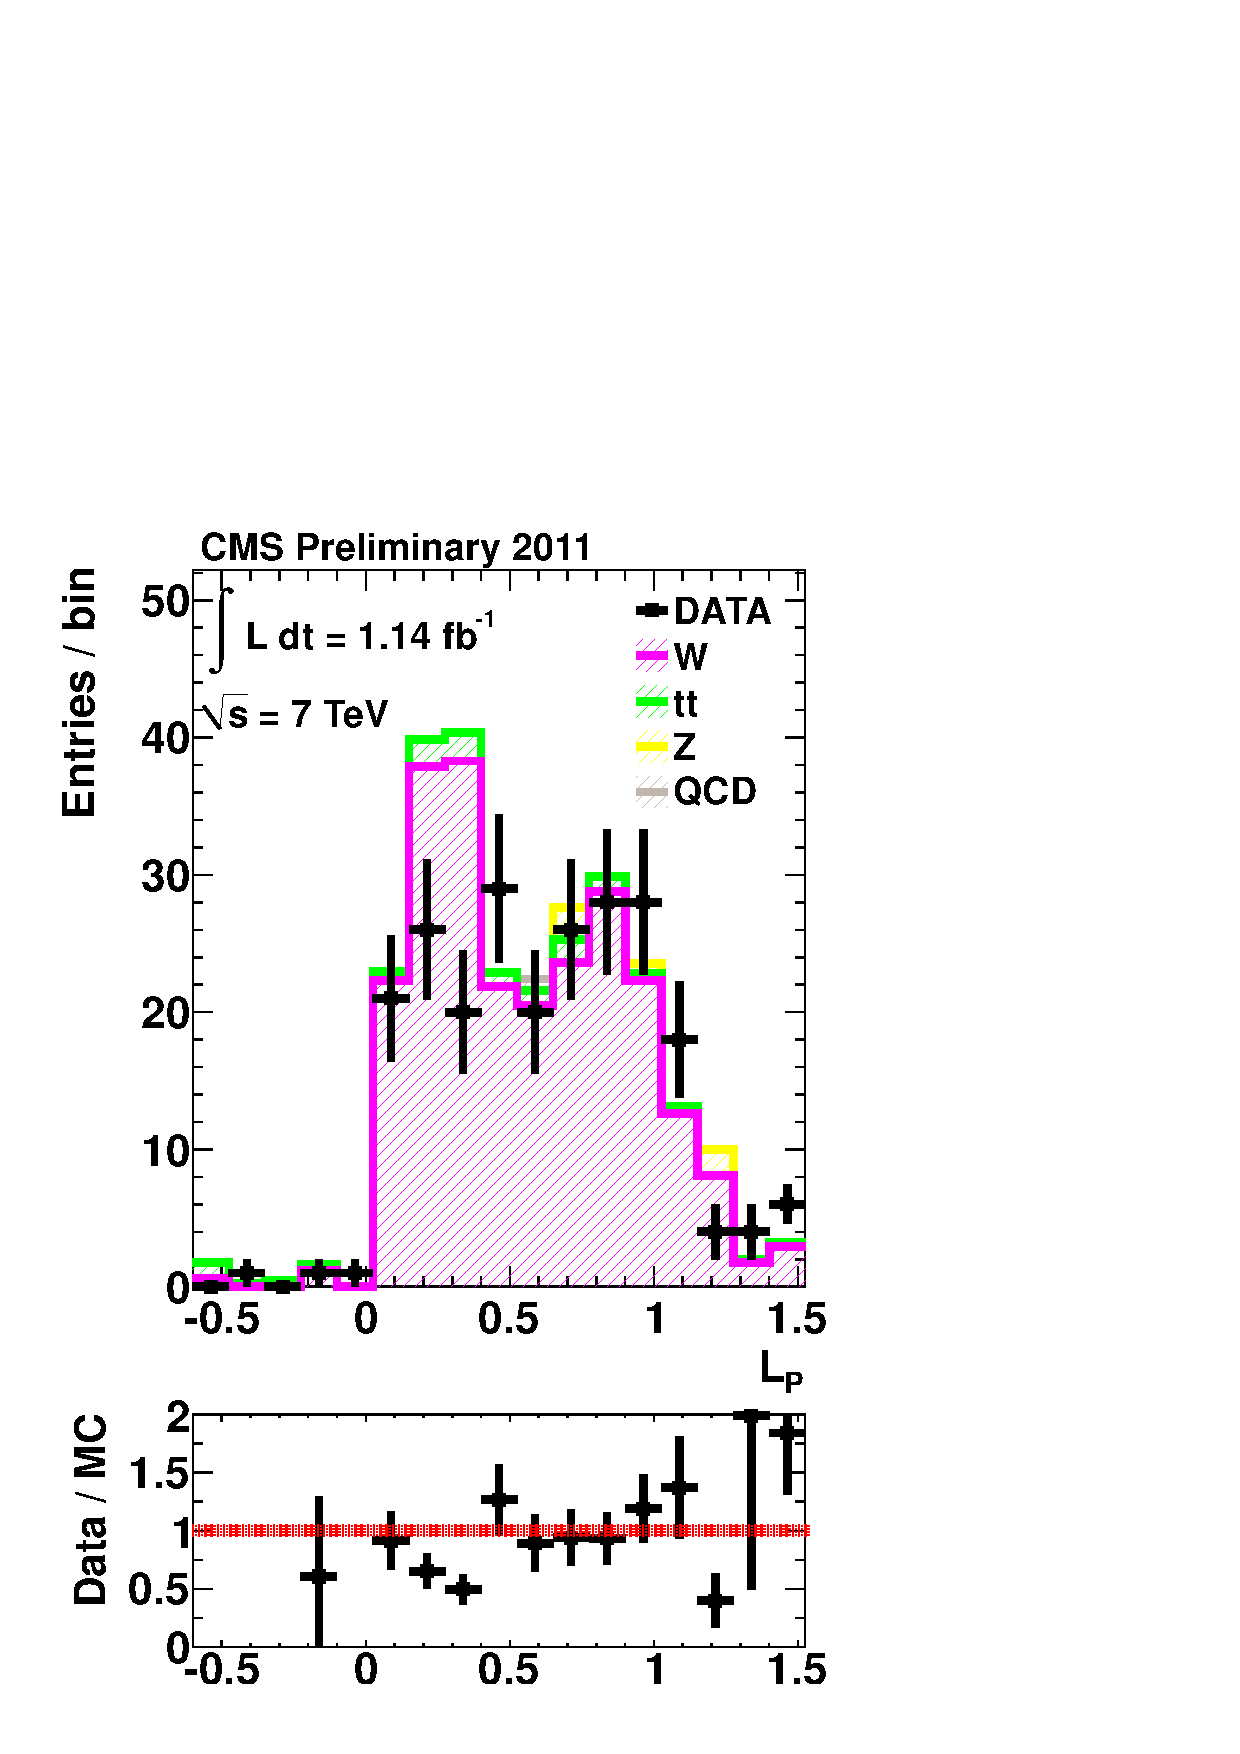
\includegraphics[width=0.3\textwidth]{fig/MuControl_LP350}}\quad
\subfloat[$\STlep > 450$]{\label{fig:susy_mucontrol_lp450}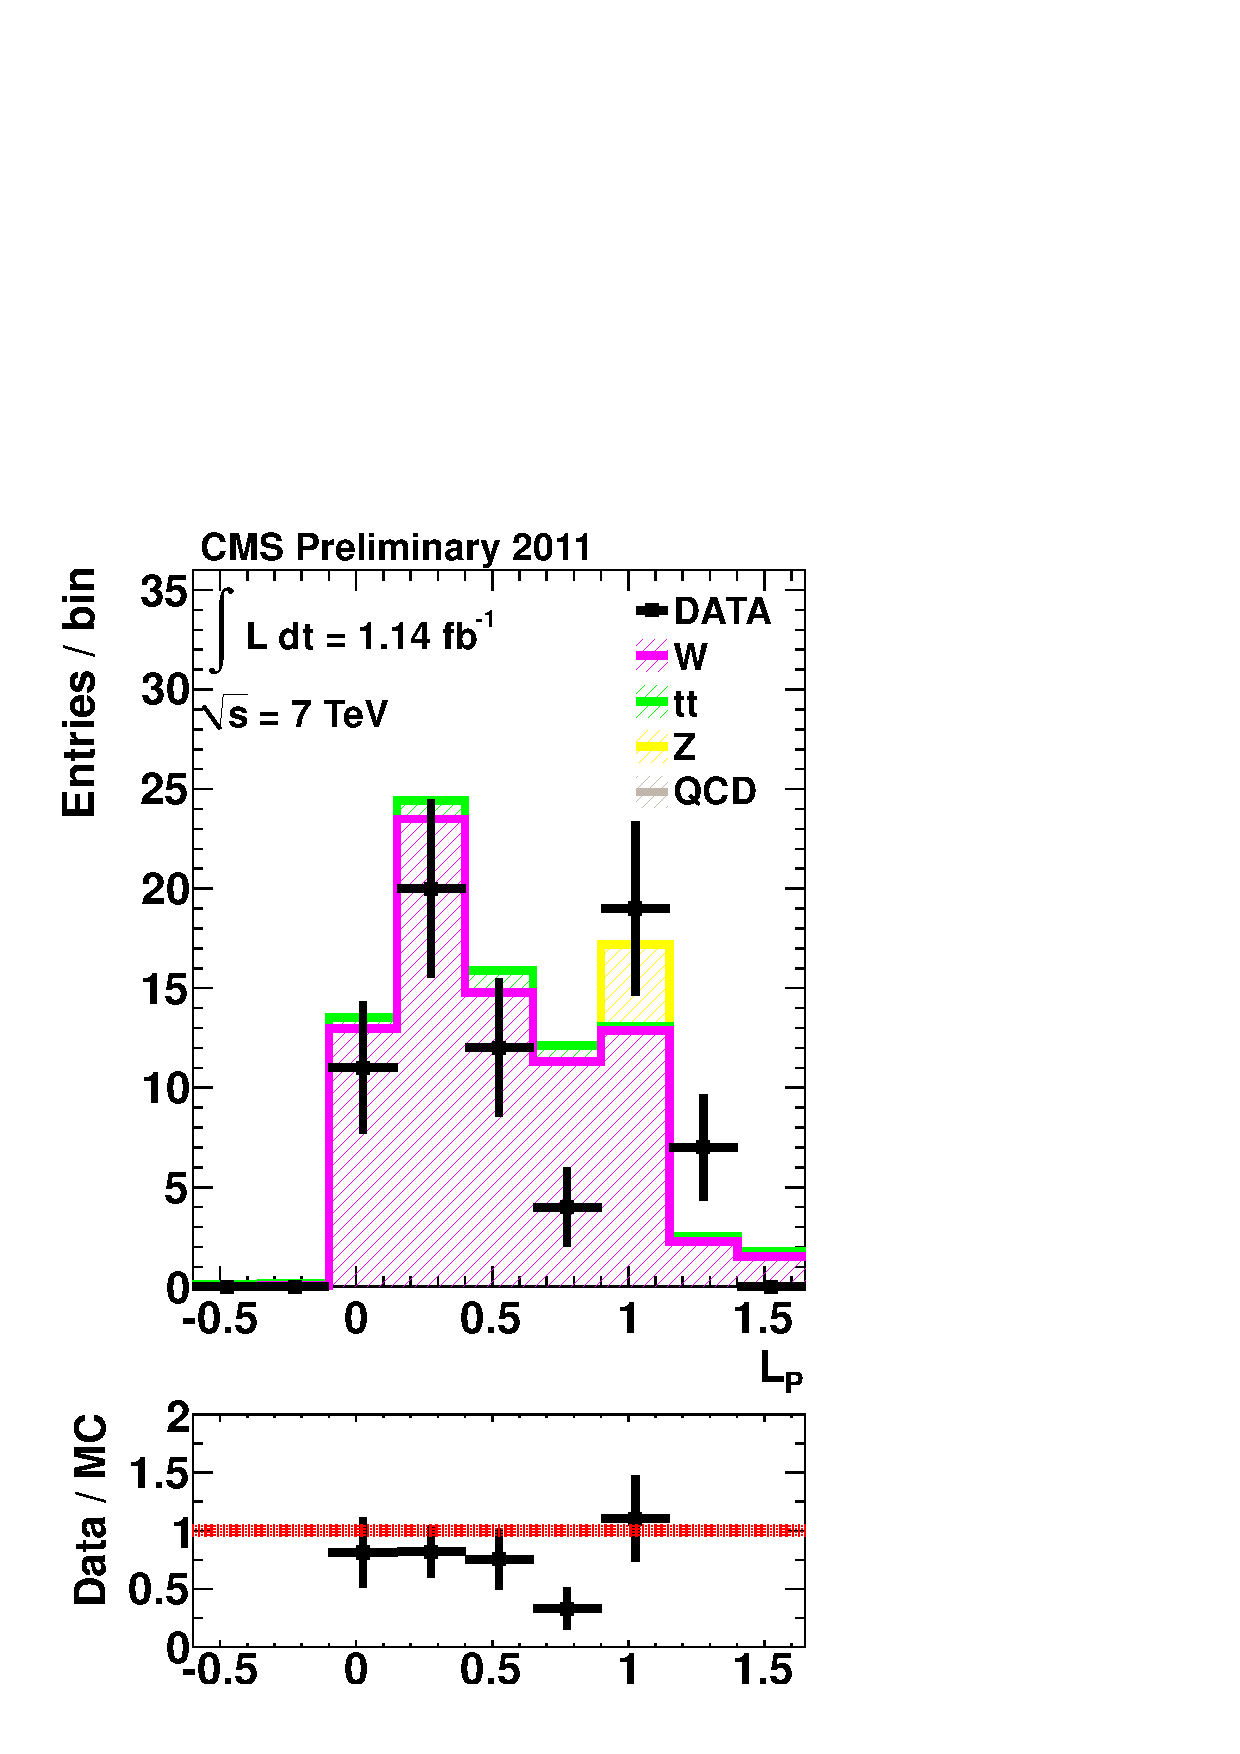
\includegraphics[width=0.3\textwidth]{fig/MuControl_LP450}}
\caption{Distribution of the \LP variable in bins of \STlep as measured in the muon control sample.}
\label{fig:susy_mucontrol_lp}
\end{figure}

\section{Background Prediction}
As for the \PW polarisation analysis, the background from \ac{QCD} multijet
events again presents a difficulty. In the muon channel, the \ac{QCD}
contribution is once again small to negligible as evidenced in
Table~\ref{tbl:susy_mcexp_control}. For this, it is sufficient to calculate
only an upper bound. For the electron channel, as before, the contribution is
much larger. Fortunately, the methods outlined in
Section~\ref{sec:wpol_data_driven_bg} prove to be effective again, with some
adaptation.

\subsection{Muons}
A conservative upper limit on the \ac{QCD} background in the muon channel is
obtained from a data-driven control sample by inverting the isolation cut, $0.2
< \CombIso < 0.5$. In order to further enrich \ac{QCD} events whilst supressing
electroweak backgrounds in this sample, a $\MET < \unit{20}{\GeV}$ cut is also
applied. Even with these cuts, significant electroweak contamination
remains. The significance of the vertex impact paramter is used as an additional
handle by requiring $\sigma(D_0) > 3$. The ratio $N(\CombIso < 0.1/N(0.2 <
\CombIso < 0.5)$ in this sample is then used to derive an upper limit on the
\ac{QCD} contribution. This limit is conservative given that electroweak
background are present in the ratio. It is seen in Table~TODO that the \ac{QCD}
background is negligible in all \STlep bins and is ignored in the subsequent
analysis.

\subsection{Electrons}
\label{sec:susy_electron_bgpredict}
In the case of the electrons, a strategy similar to that used in the \PW
polarisation analysis is employed. As before, the electron identification
variables \deltaetain and \deltaphiin are inverted. In addition, to ensure
adequate statistics the \D0 and \Dz cuts are removed and the isolation cut is
relaxed. The \D0 and \Dz cuts were not present in the \PW polarisation
selection. Although the present analysis benefits from a dataset $\sim 30$ times
larger than that used for the previous measurement, statistics are hurt by the
generally tighter kinematic cuts.

In addition, it was observed during studies for the \PW polarisation measurement
that the shape of the QCD template was affects by a cut on \PtW. Thus it should
be assumed to depend too on \STlep, necessitating the use of independent
templates for each \STlep bin. A comparison of the selected and anti-selected
shapes in simulated \ac{QCD} events is shown in Figure~\ref{fig:susy_elqcd_selasel}. This may be
compared with those derived in the \PW polarisation analysis (see
Figure~\ref{fig:wpol_ele_sel_antisel}). Differences may be accounted for by the
modified electron selection and kinematic cuts.

As in the \PW polarisation analysis, a binned maximum likelihood fit is
performed using electroweak background templates for the electroweak backgrounds
derived from simulation. To avoid the potential effects of signal contamination,
the fit region is restricted to \LPcontrol and then the fit result is used to
extrapolate into \LPsignal. The results of these fits are shown in
Figures~\ref{fig:susy_elqcd_fitresult150}
and~\ref{fig:susy_elqcd_fitresult250}. The predictions of the \ac{QCD} and
electroweak background contamination can be seen in Table~TODO. The \ac{QCD}
contamination in the signal region is seen to be negligible.

The results of the fit can be used to directly predict the background
contamination in the signal region. However, in order to compare systematic
uncertainties with the muon channel, a corrected \RCS is calculated from the fit
results. The systematic uncertainties are then calculated in terms of this
variable. For the limit procedure, it was technically simpler to use the fit
results to correct the \NControl to subtract the \ac{QCD} contribution. Since
the \ac{QCD} contamination in the signal region is negligible, this should not
make a significant difference to the limit.

To account for the \ac{QCD} contamination in the control
region, the background prediction in the electron channel is derived from the
fitted number of electroweak events. Similarly, the \RCS calculation in
simulation is performed using only the electroweak background components. The
additional uncertainties introduced by this procedure will be covered in
Section~\ref{sec:susy_systematics}.

\begin{figure}
\centering
\subfloat[Comparison of the \LP distribution between selected and anti-selected electron samples]{
  \label{fig:susy_elqcd_selasel}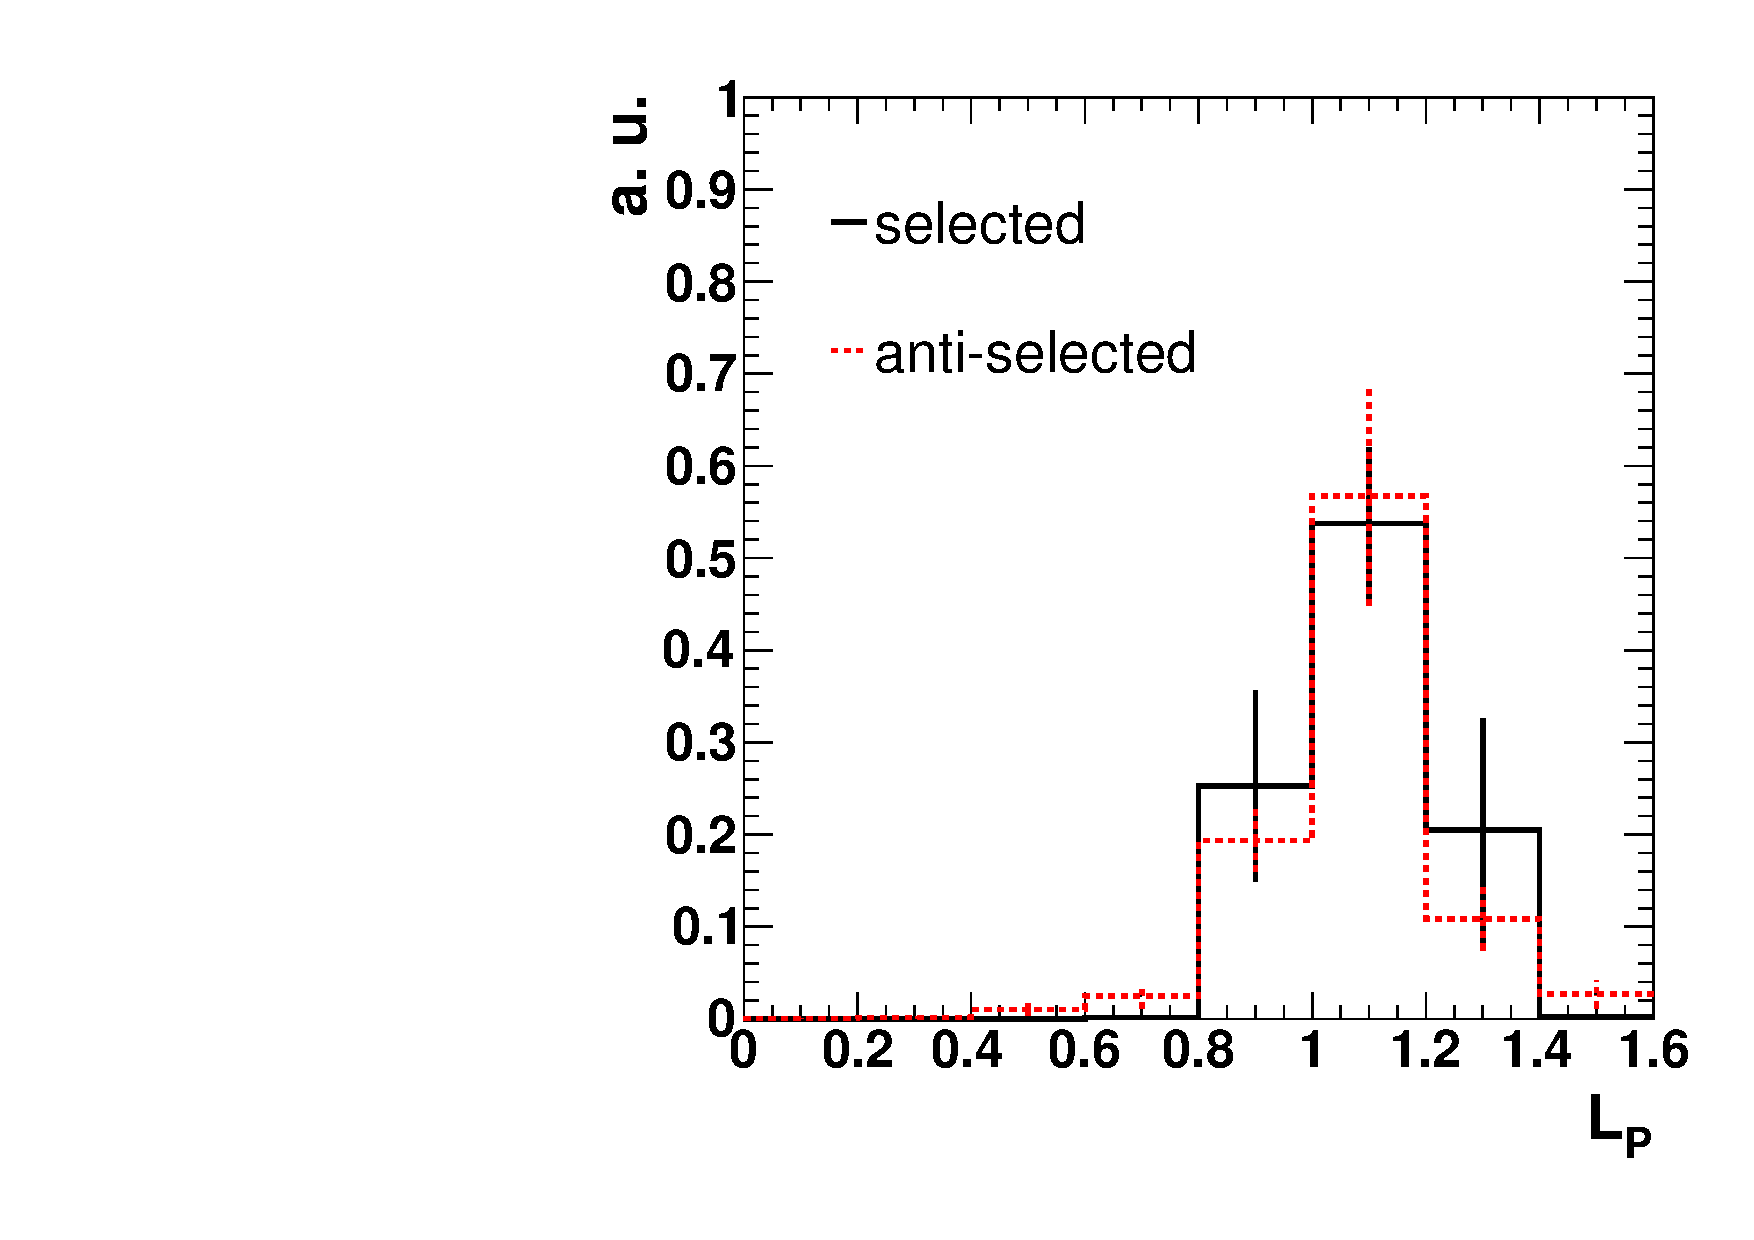
\includegraphics[width=0.5\textwidth]{fig/SelectedVsAntiSelected}}\quad\\
\subfloat[Fit results $150 < \STlep < 250$]{\label{fig:susy_elqcd_fitresult150}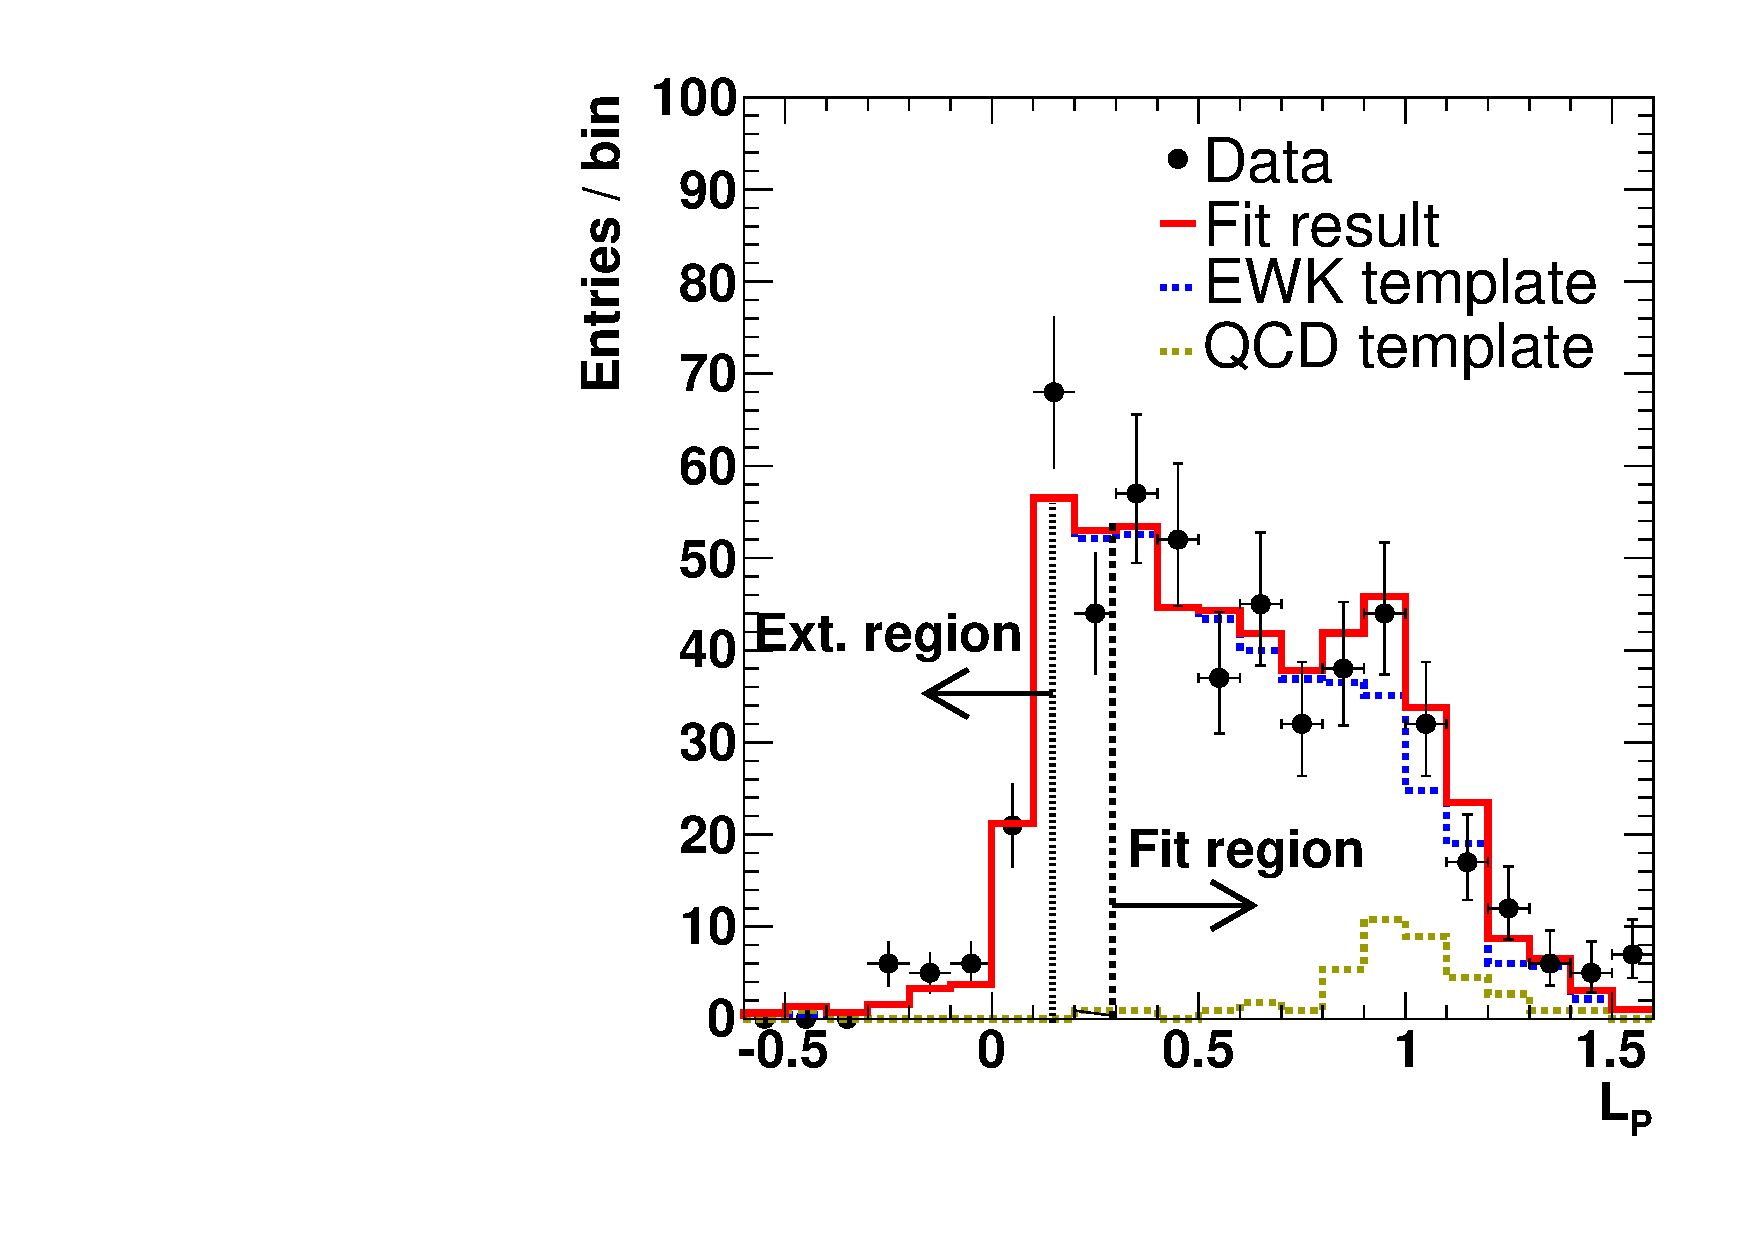
\includegraphics[width=0.4\textwidth]{fig/FitResult_El_150}}\quad
\subfloat[Fit results $250 < \STlep < 350$]{\label{fig:susy_elqcd_fitresult250}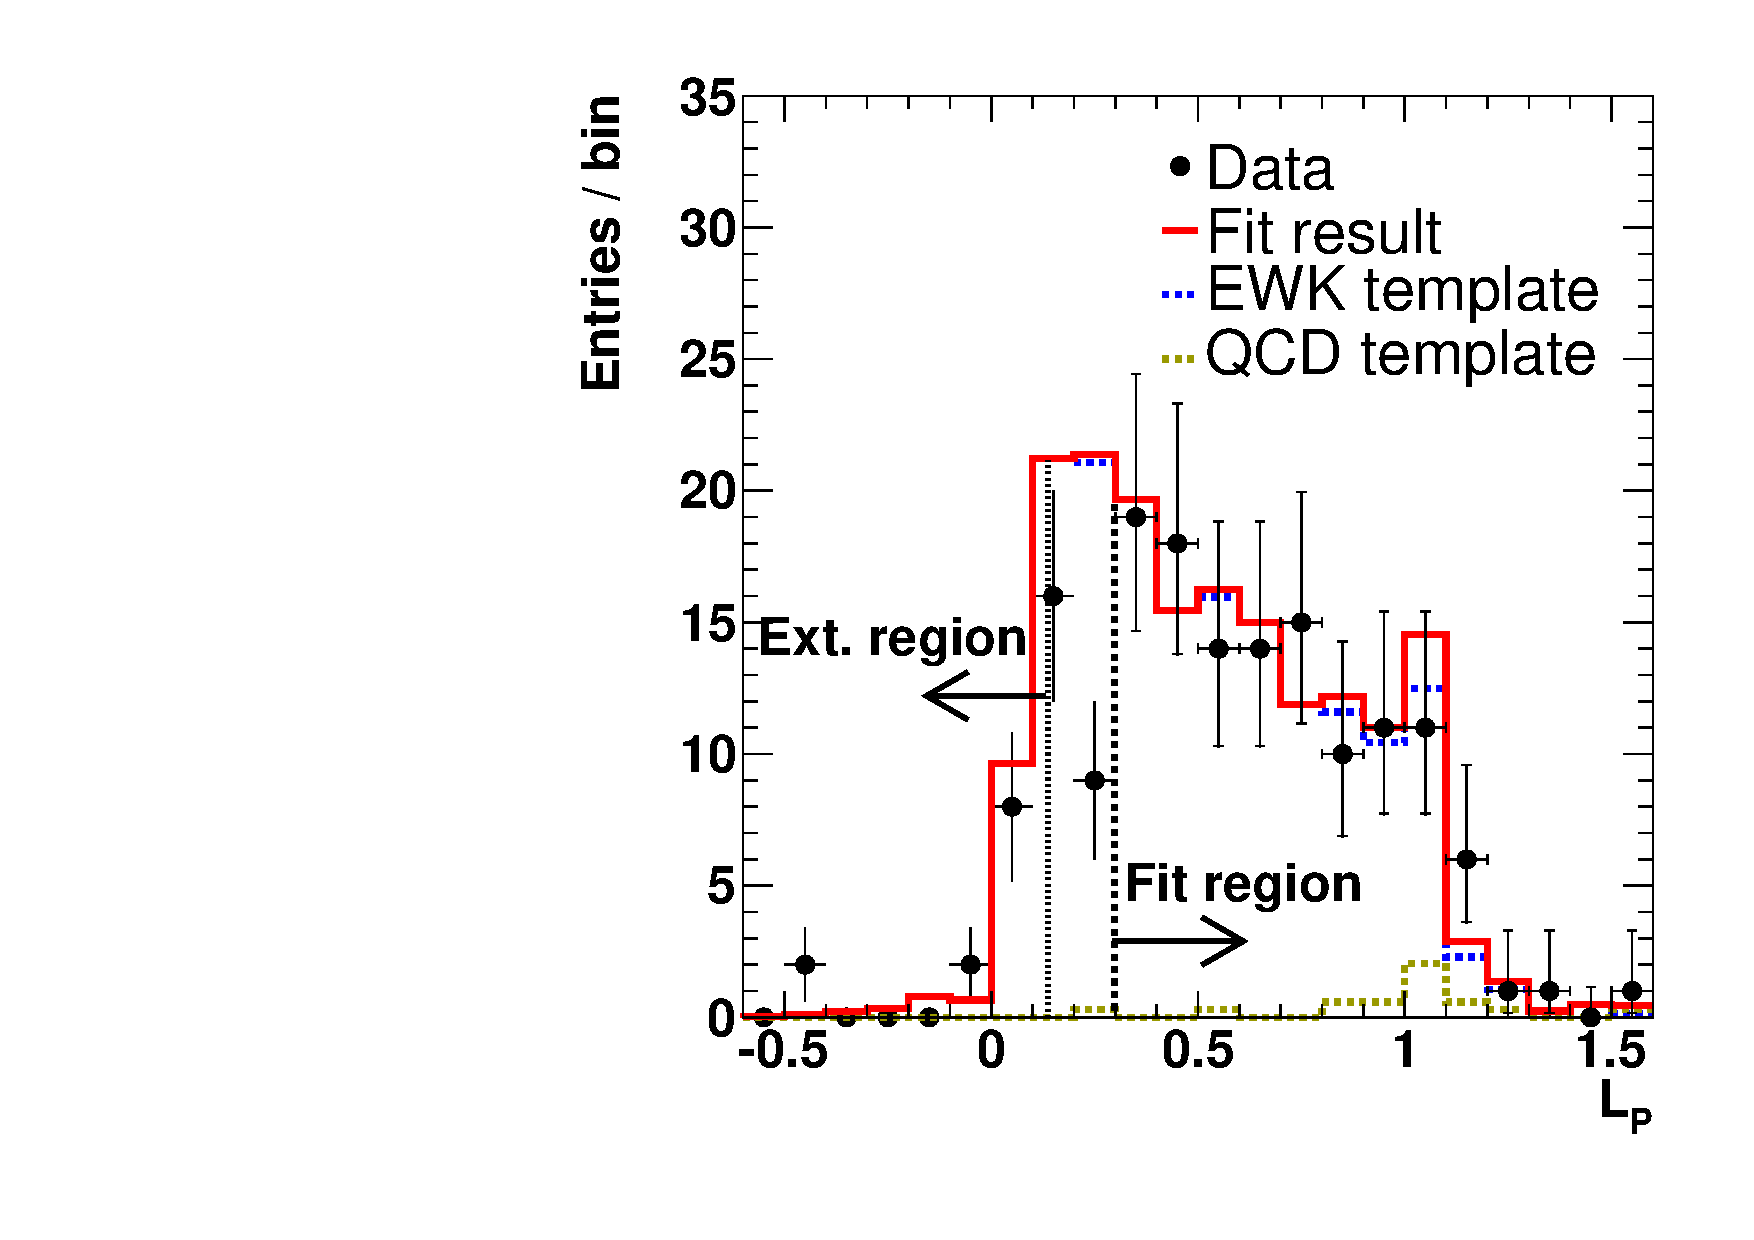
\includegraphics[width=0.4\textwidth]{fig/FitResult_El_250}}
\caption[]{Figure~\subref{fig:susy_elqcd_selasel} shows a comparison of the \LP
  shape between simulated \ac{QCD} events in the selected and anti-selected
  samples. Figures~\subref{fig:susy_elqcd_fitresult150} and
  \subref{fig:susy_elqcd_fitresult250} show the results of the data-driven fits
  in two \STlep bins.}
\label{fig:susy_elqcd}
\end{figure}

\section{Systematics}
\label{sec:susy_systematics}
For this analysis, as with the \PW polarisation measurement, unavoidable
dependence on simulation requires careful evaluation of associated systematic
uncertainties. It has already been said that the construction of \RCS is
intended to minimise some of these uncertainties by ensuring some degree of
cancellation. Experience from the \PW polarisation measurement showed that the
\LP variable is highly sensitive to certain uncertainties - in particular the
jet energy scale. The size of these uncertainties was thus evaluated early-on in
the development of the analysis and continued throughout. Several of the
systematics procedures were adopted or adapted from those used for the previous
measurement (see Section~\ref{sec:wpol_systematics}).

The background prediction procedure may be written as follows,
\begin{equation}
\NBkgi = \RCSi \times \NControli
\end{equation}
where \NBkgi is the predicted background for \LPsignal in \STlep bin $i$, \RCSi
the corresponding translation factor and \NControli the expected electroweak
yield in the region \LPcontrol (i.e. for the muons, simply the event yield
assuming zero contamination from \ac{QCD} or for electrons, the result of the
fit described in Section~\ref{sec:susy_electron_bgpredict}).

The uncertainty assigned to the background prediction \NBkg must come from two
sources: uncertainty on the translation factor, \RCS and uncertainty on the yield
in the control region, \NControl. These sources of uncertainty will now be
described.

\subsection{Limited Statistics in the Control Region \texorpdfstring{\LPcontrol}{\LPcontrolBM}}
The effect of finite statistics in the control region is naturally more
pronounced in the larger \STlep bins. For the muon channel, this is simply
calculated as the Poisson uncertainty ($\sqrt{N}$) of the number of events in
the control region. For electrons, this uncertainty is taken as the error on the
fitted electroweak component of the background.

\subsection{Limited Monte Carlo Statistics}
\label{sec:susy_syst_mcstats}
The limited statistics of simulated events results in an uncertainty for both
channels in the calculation of \RCS. This is calculated by simple propagation of
errors.

For the electron channel, things are once again complicated by the \ac{QCD}
fitting procedure. The electroweak templates used in the fit also suffer from
limited statistics, thus leading to an additional source of uncertainty on
\NControl. This is accounted for in a similar manner to the statistical
uncertainty of the \ac{QCD} template in the \PW polarisation analysis (see
Section~\ref{sec:wpol_syst_ele_bgest}. The templates are rediced 200 times
according to the statistical error per bin. Each rediced template is then used
to repeat the fit procedure. The variance of this ensemble of fits is then taken
to be the statistical uncertainty. For the systematics quoted in
Table~\ref{tbl:susy_syst_muons}, this is propagated into \RCS. For the limit, as
will be seen, it is taken as an uncertainty on \NControl.

\subsubsection{Jet Energy Scale Uncertainty}
\label{sec:susy_jes_uncertainty}
This procedure was changed with respect to the \PW polarisation measurement in
order to harmonise with other analyses. Each jet in the event, as well as the
remaining hadronic recoil are scaled upwards or downwards by 5\%. The larger of
the two shifts on \RCS is then taken as the uncertainty. If the the uncertainty
is found to be smaller than the Monte Carlo statistical error
(Section~\ref{sec:susy_syst_mcstats}), the uncertainty is taken to be the larger
of the two.

\subsubsection{Hadronic Recoil Resolution}
\label{sec:susy_metres_uncertainty}
The resolution of the hadronic recoil has previously been measured
in~\cite{cms_met_pas}. The resolution measured in data is seen to be 10\% larger
than predicted by simulation. To account for this, the recoil is smeared by an
additional 10\% perpendicular and parallel to its direction. The resulting shift
in \RCS is taken as the uncertainty.

\subsubsection{\Wjets/\ttbar Cross Section}
Te use of \RCS avoids any dependence on the absolute values of theoretical
cross-sections. However, since the \Wjets and \ttbar lead to different \LP
shapes, changes to their relative normalisations will result in changes to
\RCS. To account for this, the \Wjets and \ttbar contributions are each scaled
up and down by 30\% and 50\% respectively. The shift in \RCS with respect to the
unscaled case is then calculated. The shifts are performed simultaneously to
give the most extreme change in \RCS, i.e. one cross-section is shifted up, the
other down. The largest such shift is taken as the uncertainty. As for the jet
energy scale, a shift smaller than the statistical uncertainty of the simulated
sample is taken to be the same as the statistical uncertainty. Additionally, the
uncertainty is calculated simulatenously for both lepton channels in order to
maximise available statistics.

\subsubsection{Muon Momentum Scale}
A bias on the muon momentum is introduced. This is found to be 1\% from studies
of the \PZ mass.

\subsubsection{\PW and \ttbar Polarisation}
The polarisation in \ttbar events is found to be 5\%. Since the effect on \RCS
is less than 5\%, this is assigned as a conservative uncertainty.

For the \PW polarisation, the errors on the previous measurement were taken and
used to assign a 15\% uncertainty to the difference of the left-handed and
right-handed fractions \fLmfR (see Section~\ref{sec:wpol_results}). To account
for this, the simulation was reweighted to reflect and upward and downard shift
of 15\% on \fLmfR with respect to the nominal values. This is done in a manner
similar to that used for the actual measurement (see
Section~\ref{sec:wpol_reweighting}), but using 5 bins in \PtW instead of 3. The
results are shown for the highest \STlep bin in
Figure~\ref{fig:susy_wpol_syst}. The largest of the two shifts is taken to be
the systematic uncertainty.

\begin{figure}
\centering
\subfloat[]{\label{fig:susy_wpol_syst_plus}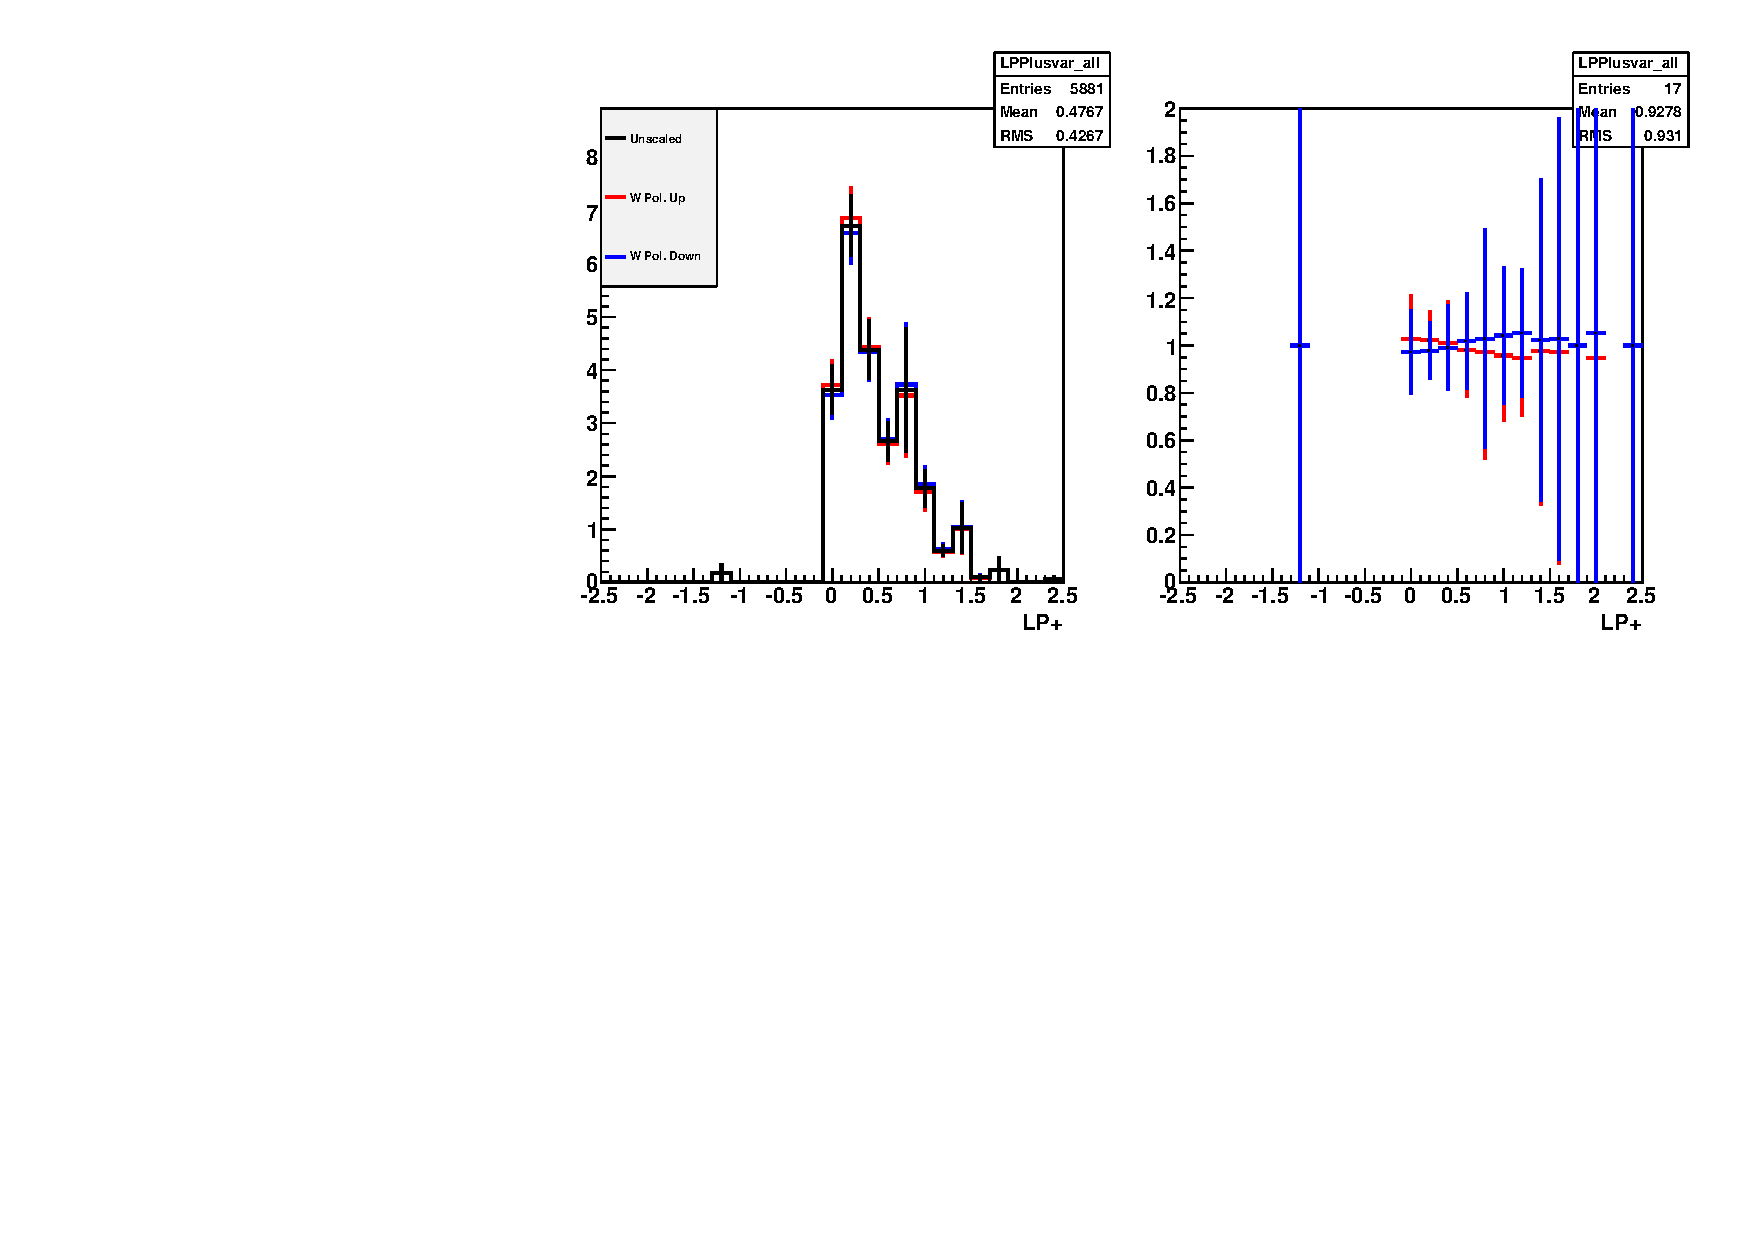
\includegraphics[width=0.9\textwidth]{fig/MuonStandardPlots_450_NOLP_LPPlusvar_all_ratio}}\\
\subfloat[]{\label{fig:susy_wpol_syst_minus}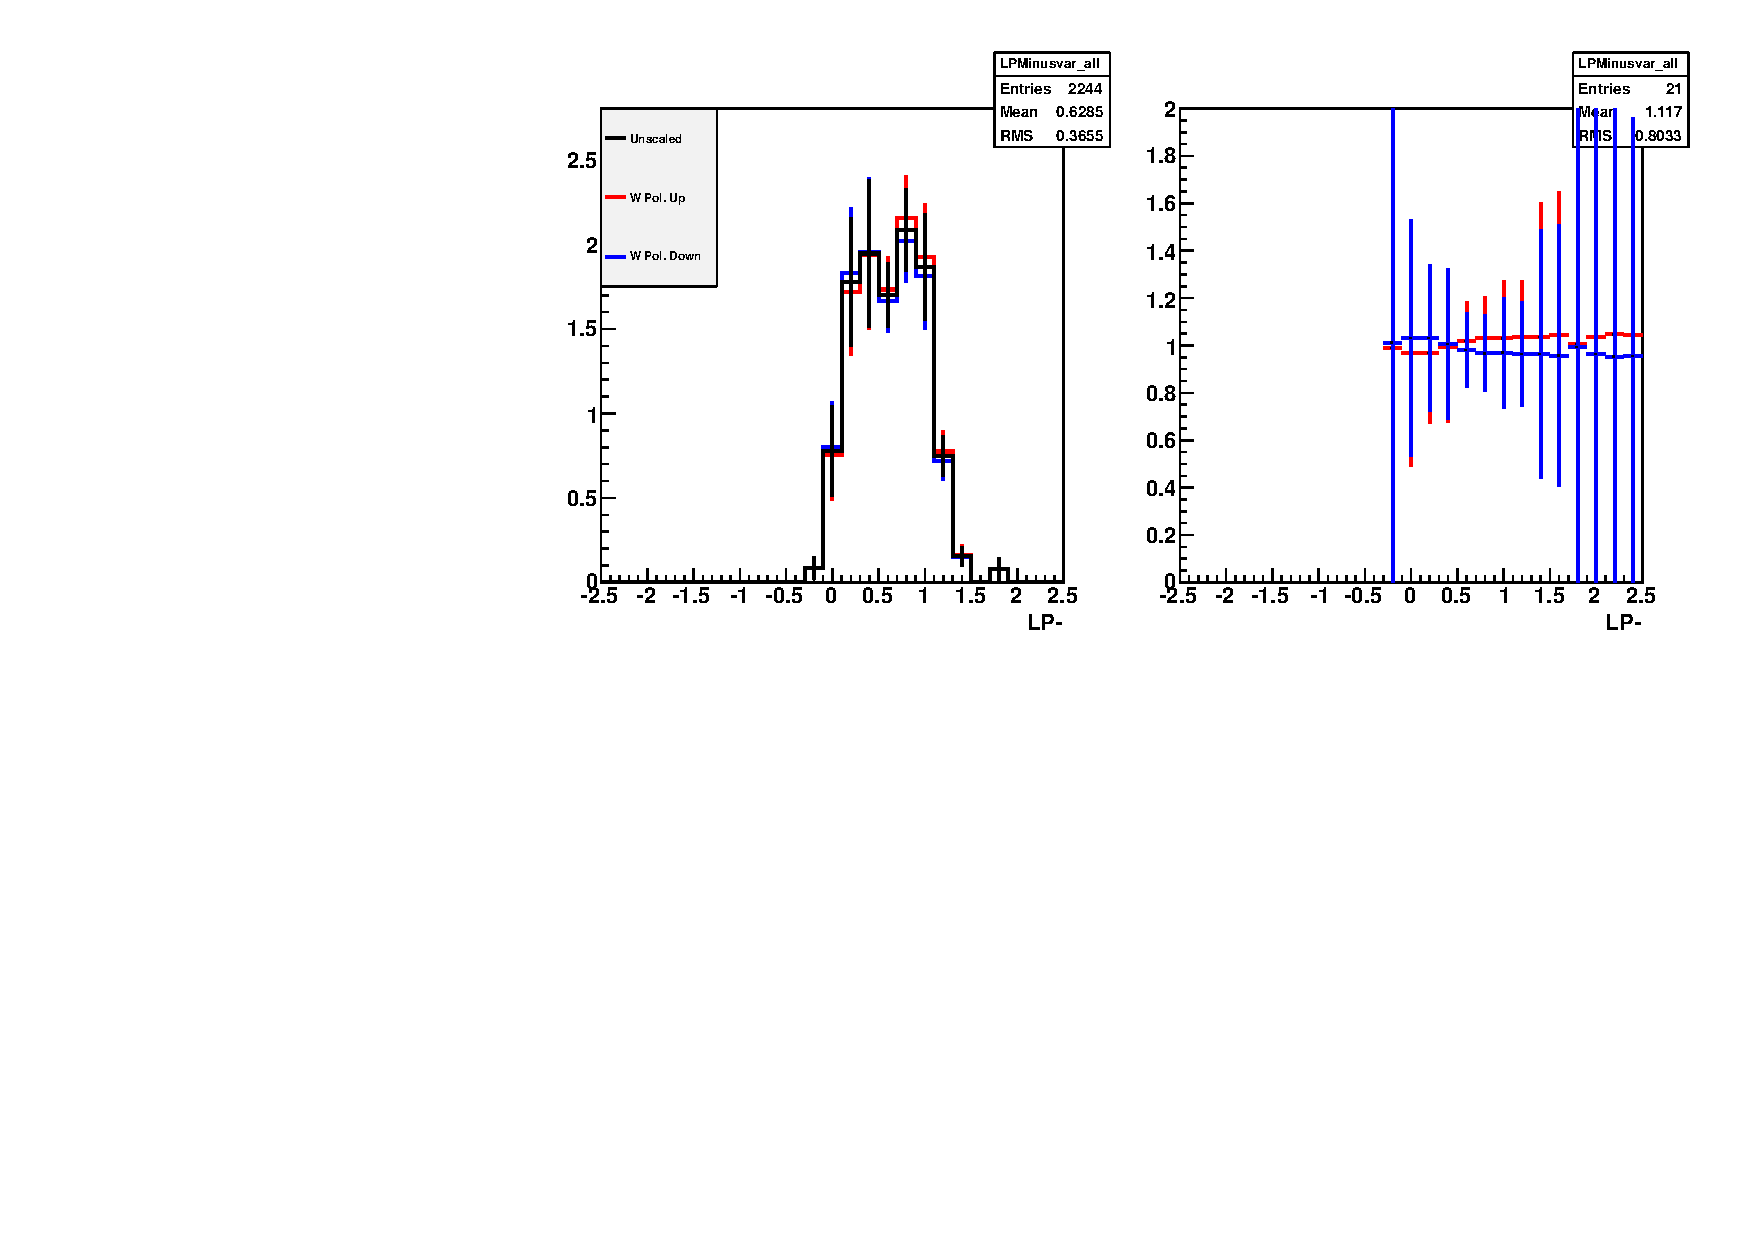
\includegraphics[width=0.9\textwidth]{fig/MuonStandardPlots_450_NOLP_LPMinusvar_all_ratio}}
\caption[]{Shown on the left are the \LP distributions for: no change to the \PW
  polarisation (black), an upward shift of 15\% on \fLmfR (red) and a downard
  shift of 15\% on \fLmfR (blue). Right hand plots show the corresponding
  ratios. Upper plots are for positive charged muons, lower plots for negatively charged muons.}
\label{fig:susy_wpol_syst}
\end{figure}

\subsubsection{Fully Leptonic \ttbar}
The fraction of events passing the selection in which a second lepton is not
identified, either due to reconstruction or acceptance effects, is estimated in
simulation. Since this is a relatively small fraction of the background, a
conservative 50\% uncertainty is assumed. The resulting change in the \LP shape
is then propagated into \RCS.

\subsubsection{\acl{PDF} Uncertainties}
The uncertainty stemming from the choice of \acp{PDF} was handled slightly
differently to the \PW polarisation case. The Monte Carlo was reweighted to the
central value of both CTEQ66 and MSTW2008NLO68CL \ac{PDF} sets and the resulting
change in \RCS was found to be 1\% for $\STlep < \unit{450}{\GeV}$ and 5\% for
$\STlep > \unit{450}{\GeV}$. This systematic uncertainty is therefore seen to be
negligible.

\subsubsection{Trigger Efficiency}
Whilst the efficiencies of the trigger are found to be uncorrelated with the
lepton \Pt, an $\eta$ dependence is observed. This variation is found to be 18\%
in the muon channel and 5\% in the electron channel. In addition, at the plateau
of the trigger turn-on curve, a difference of efficiency between data and
simulation is observed: 5\% in the muon channel and $\approx 1\%$ for
electrons. To estimate the combined effect of the $\eta$ dependence and the
discrepancy between data and Monte Carlo, the HLT\_Mu15 trigger is applied in
simulation. The effect on \RCS is seen to be $<1\%$ across all $\eta$ bins.

The relative uncertainties on \RCS for each significant systematic effect listed
above are shown in Table~\ref{tbl:susy_syst_muons} for the muon channel and
\ref{tbl:susy_syst_electrons} for electrons. The relative uncertainty on the
estimated number of events due to limited statistics in the control region is
also shown for comparison.

\ctable[
  caption=The relative effects on the values of \f0 and \fLmfR in the muon channel for the uncertainties described. The absolute values are shown in brackets.,
  label=tbl:wpol_mu_syst,
  doinside=\scriptsize
]{ c  p{2.5cm}  p{2.7cm}  p{2.5cm}  p{2.7cm}}{
}{\FL
     Uncertainty                         & $\fLmfR^{-}$                 & $\f0^{-}$                            & $\fLmfR^{+}$                & $\f0^{+}$ \ML
     \ac{JES}                            & $\pm11$\% (0.029)              & $\pm56$\% (0.123)       & $\pm3$\% (0.011)   & $\pm42$\% (0.092) \NN
     \MET Resolution                     & $\pm4$\% (0.012)               & $\pm3$\% (0.006)        & $\pm4$\% (0.012)   & $\pm2$\% (0.004)                        \NN
     $P_T(\mu)$ bias: $\pm$1\%/100 GeV   & $\mp$0.8\% (0.002)             & $\mp$ 11\% (0.004)      & $\pm1.2$\% (0.004) & $\mp$16.0\% (0.036)                   \ML
     Quadratic sum                       & $\pm12$\% (0.031)              & $\pm56$\% (0.123)       & $\pm5$\% (0.017)   & $\pm45$\% (0.099) \LL
}
\ctable[
cap=Systematic uncertainties in the electron channel,
caption={Sources of systematic uncertainty and their effect on the translation
factor, $R_{CS}$, in the electron channel. The relative uncertainty on the estimated number of events in the
signal region, stemming from the limited yield in the control
region, is also listed.},
pos=ht,
label=tbl:susy_syst_electrons
]{lcccc}{
}{\FL
                                   & \multicolumn{4}{c}{  \STlep Range (GeV) }\ML
                                   & [150-250] & [250-350] & [350-450] & $>$ 450\ML
$R_{CS}$                           & 0.16      & 0.18      & 0.19      & 0.23\ML
%$\Delta N/N$ at 1.1~fb$^{-1}$ (\%) & 12        & 22        & 38        & 58\ML
Systematic Uncertainty (\%)        & 14        & 20        & 24        & 34 \ML
Control Region Stat.      (\%)     & 5         & 9         & 17        & 24\NN
MC Stat.       (\%)                & 1         & 10        & 7         & 8 \NN
\ac{JES} (Flat 5\%)(\%)            & 9         & 10        & 10        & 19 \NN
\MET Resolution (10\%) (\%)         & 2         & 2         & 5         & 7 \NN
W/\ttbar Ratio (\%)                & 6         & 7         & 6         & 10 \NN
\ttbar($\ell\ell$) (\%)            & 6         & 7         & 6         & 2\NN
W Polarization (\%)                & 1         & 1         & 2         & 3\NN
\ttbar Polarization (\%)           & 5         & 5         & 5         & 5 \LL
}

\section{Results}
Once the analysis procedure had been finalised, the search region was
``unblinded''. The \LP distributions in data, along with the expected shapes in
Monte Carlo are shown in Figure~\ref{fig:susy_datamc} for the three \STlep bins
considered for the search. The predicted and observed background yields are then
shown in Table~\ref{tbl:susy_datamc_muons} for muons and
\ref{tbl:susy_datamc_electrons} for electrons. Comparison of the predicted and
observed numbers are shown graphically in Figure~\ref{fig:susy_pred}. It is
clear, that no significant excess is seen. In the next chapter, the results are
used to set limits on allowed parameter space for the \ac{CMSSM} and more
general models.
\begin{figure}
\centering
\subfloat[\Pmu $250 < \STlep < 350$]{\label{fig:susy_mu_lp250}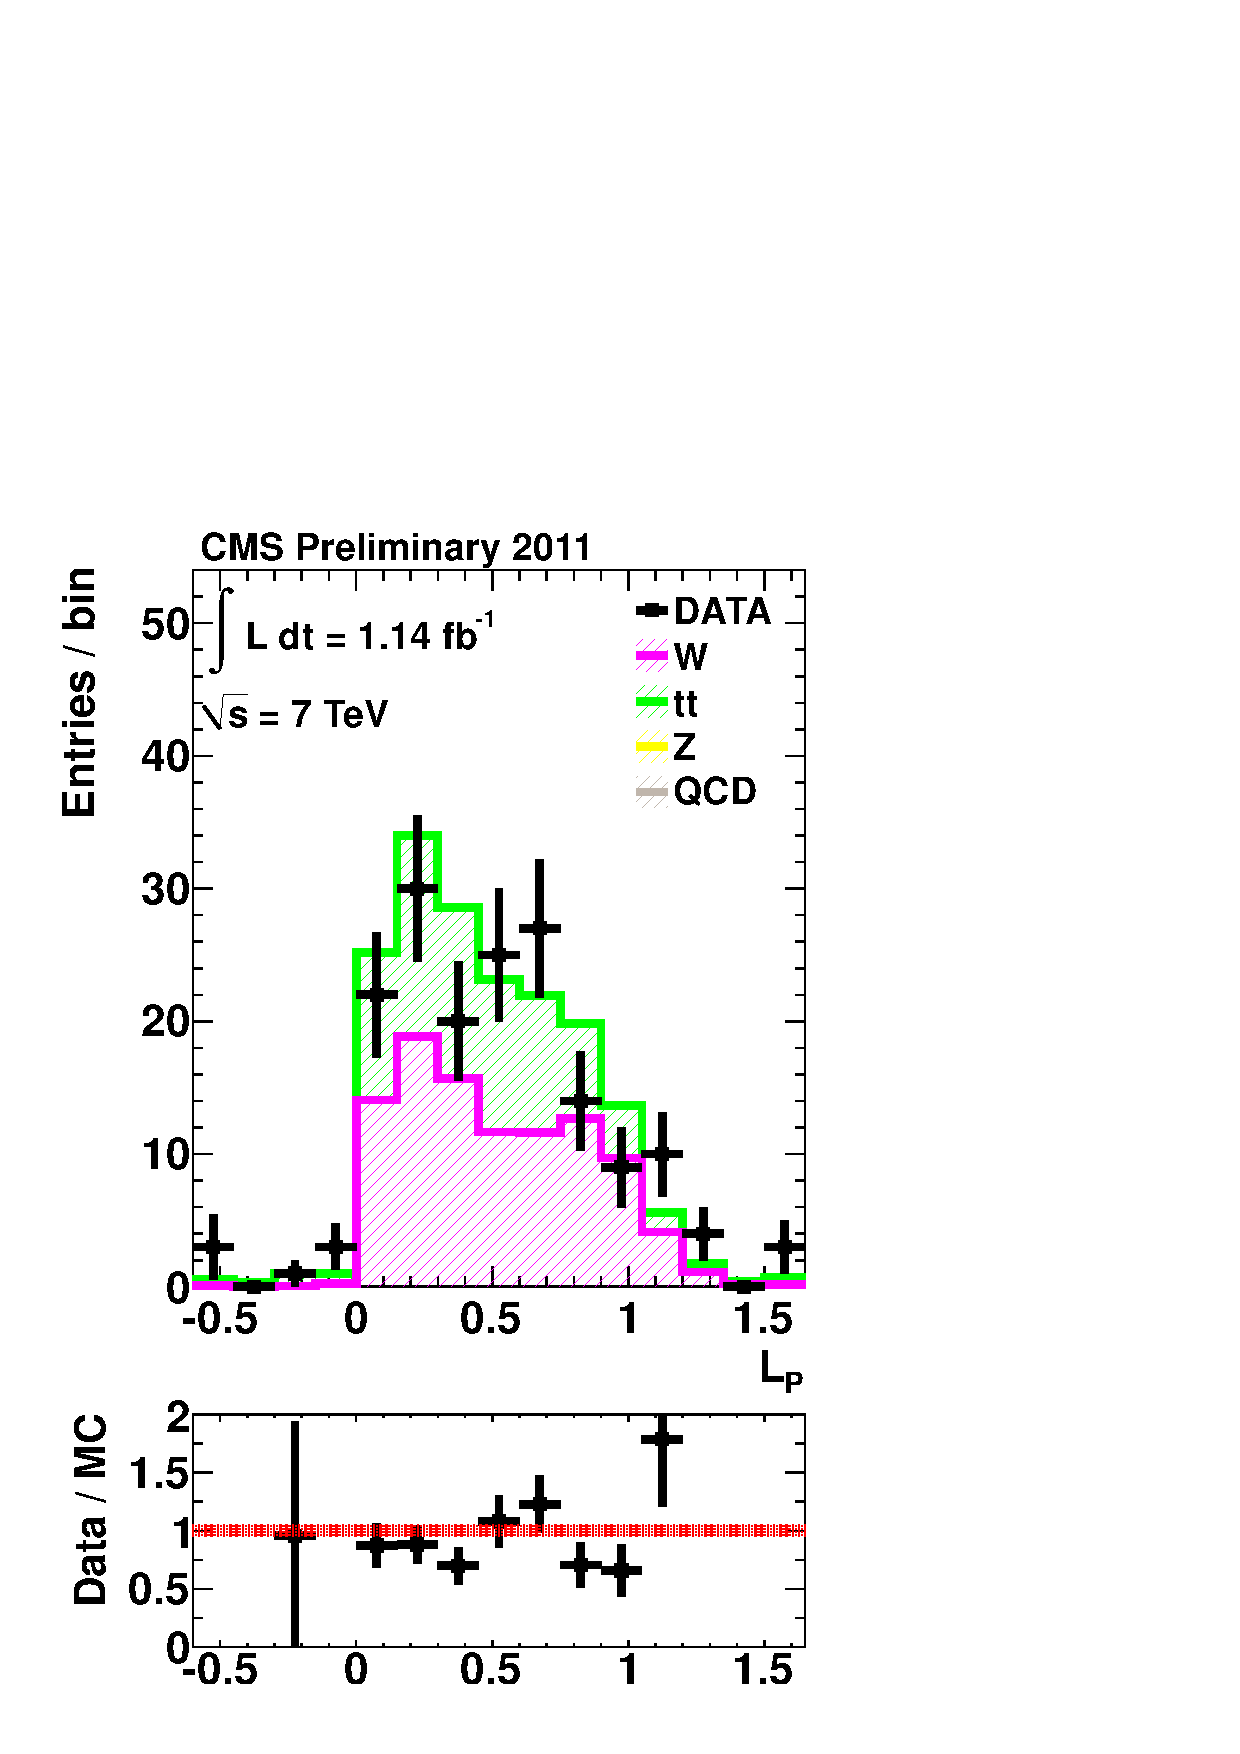
\includegraphics[width=0.3\textwidth]{fig/MuHad_LP250}}\quad
\subfloat[\Pmu $350 < \STlep < 450$]{\label{fig:susy_mu_lp350}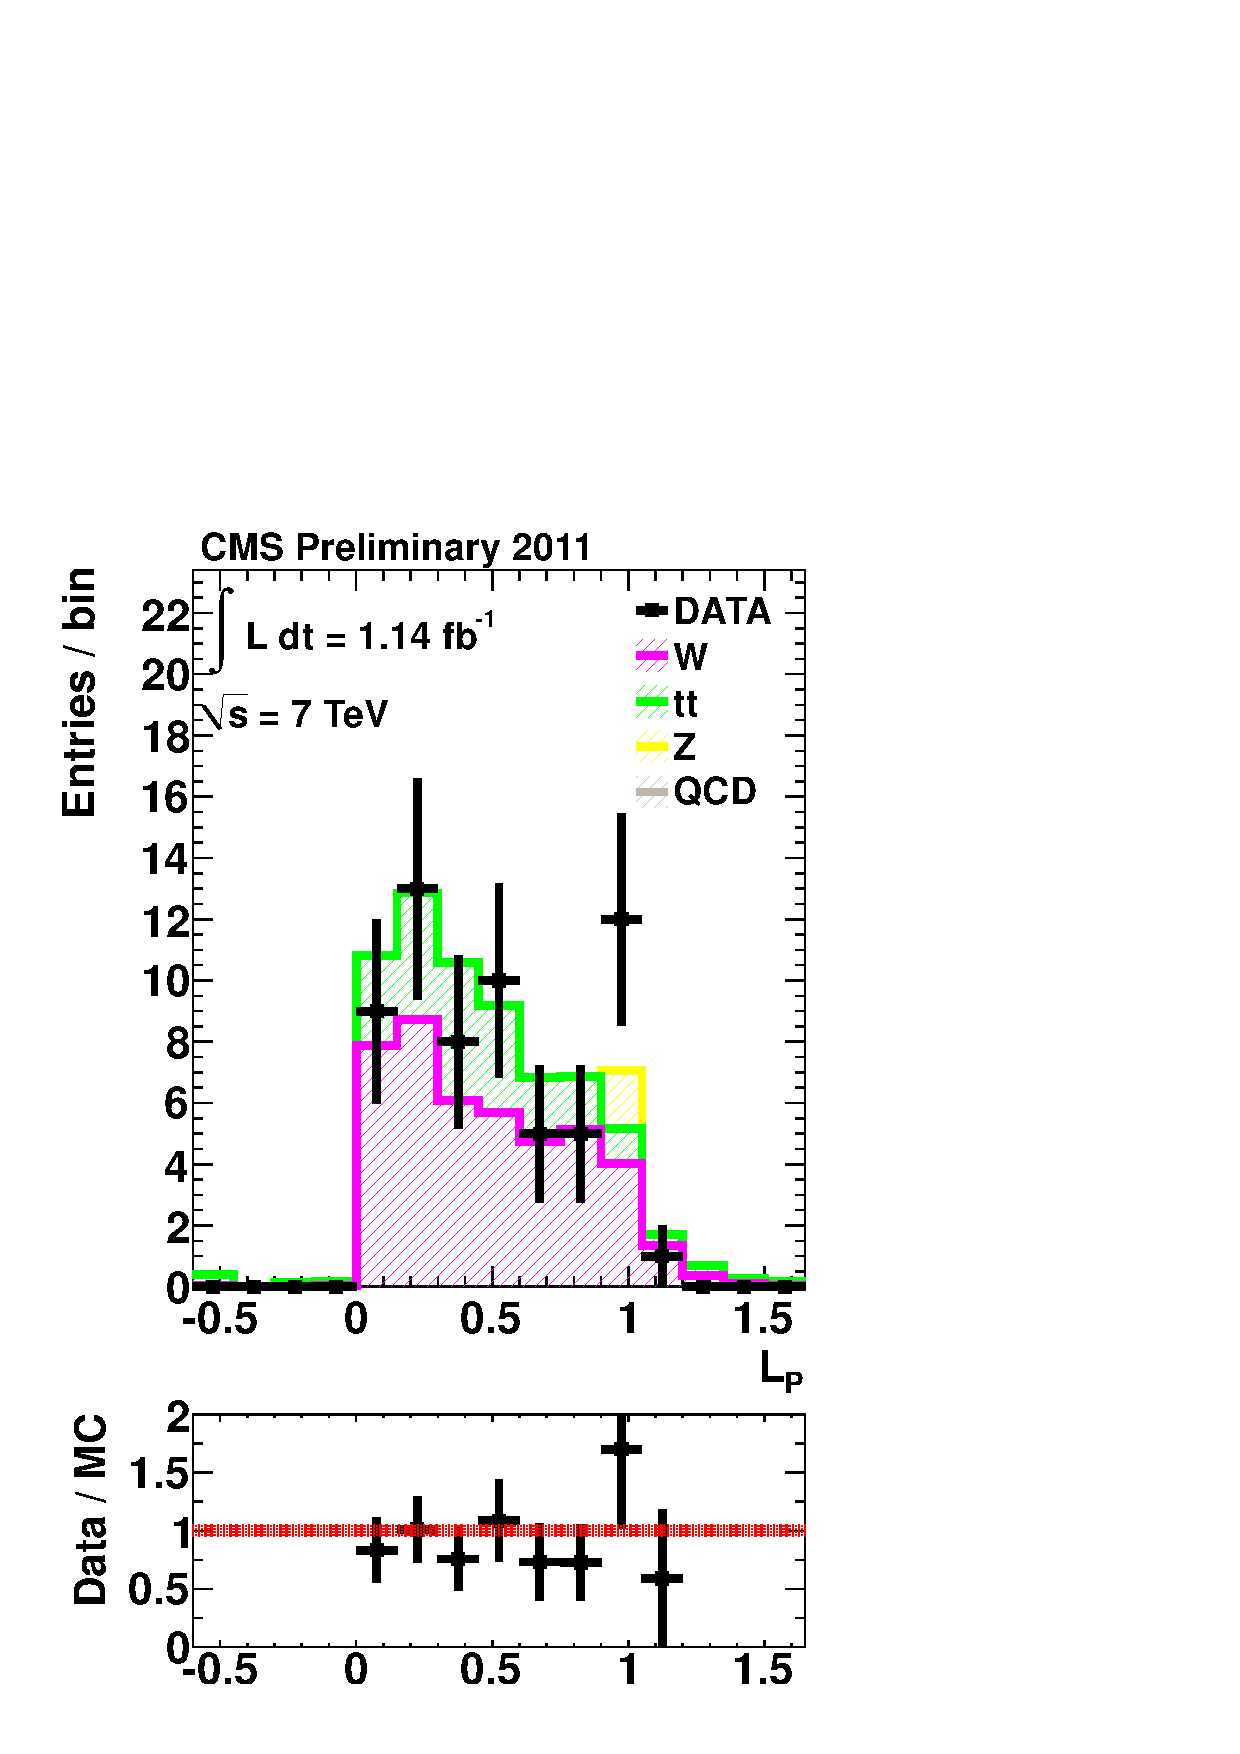
\includegraphics[width=0.3\textwidth]{fig/MuHad_LP350}}\quad
\subfloat[\Pmu $\STlep > 450$]{\label{fig:susy_mu_lp450}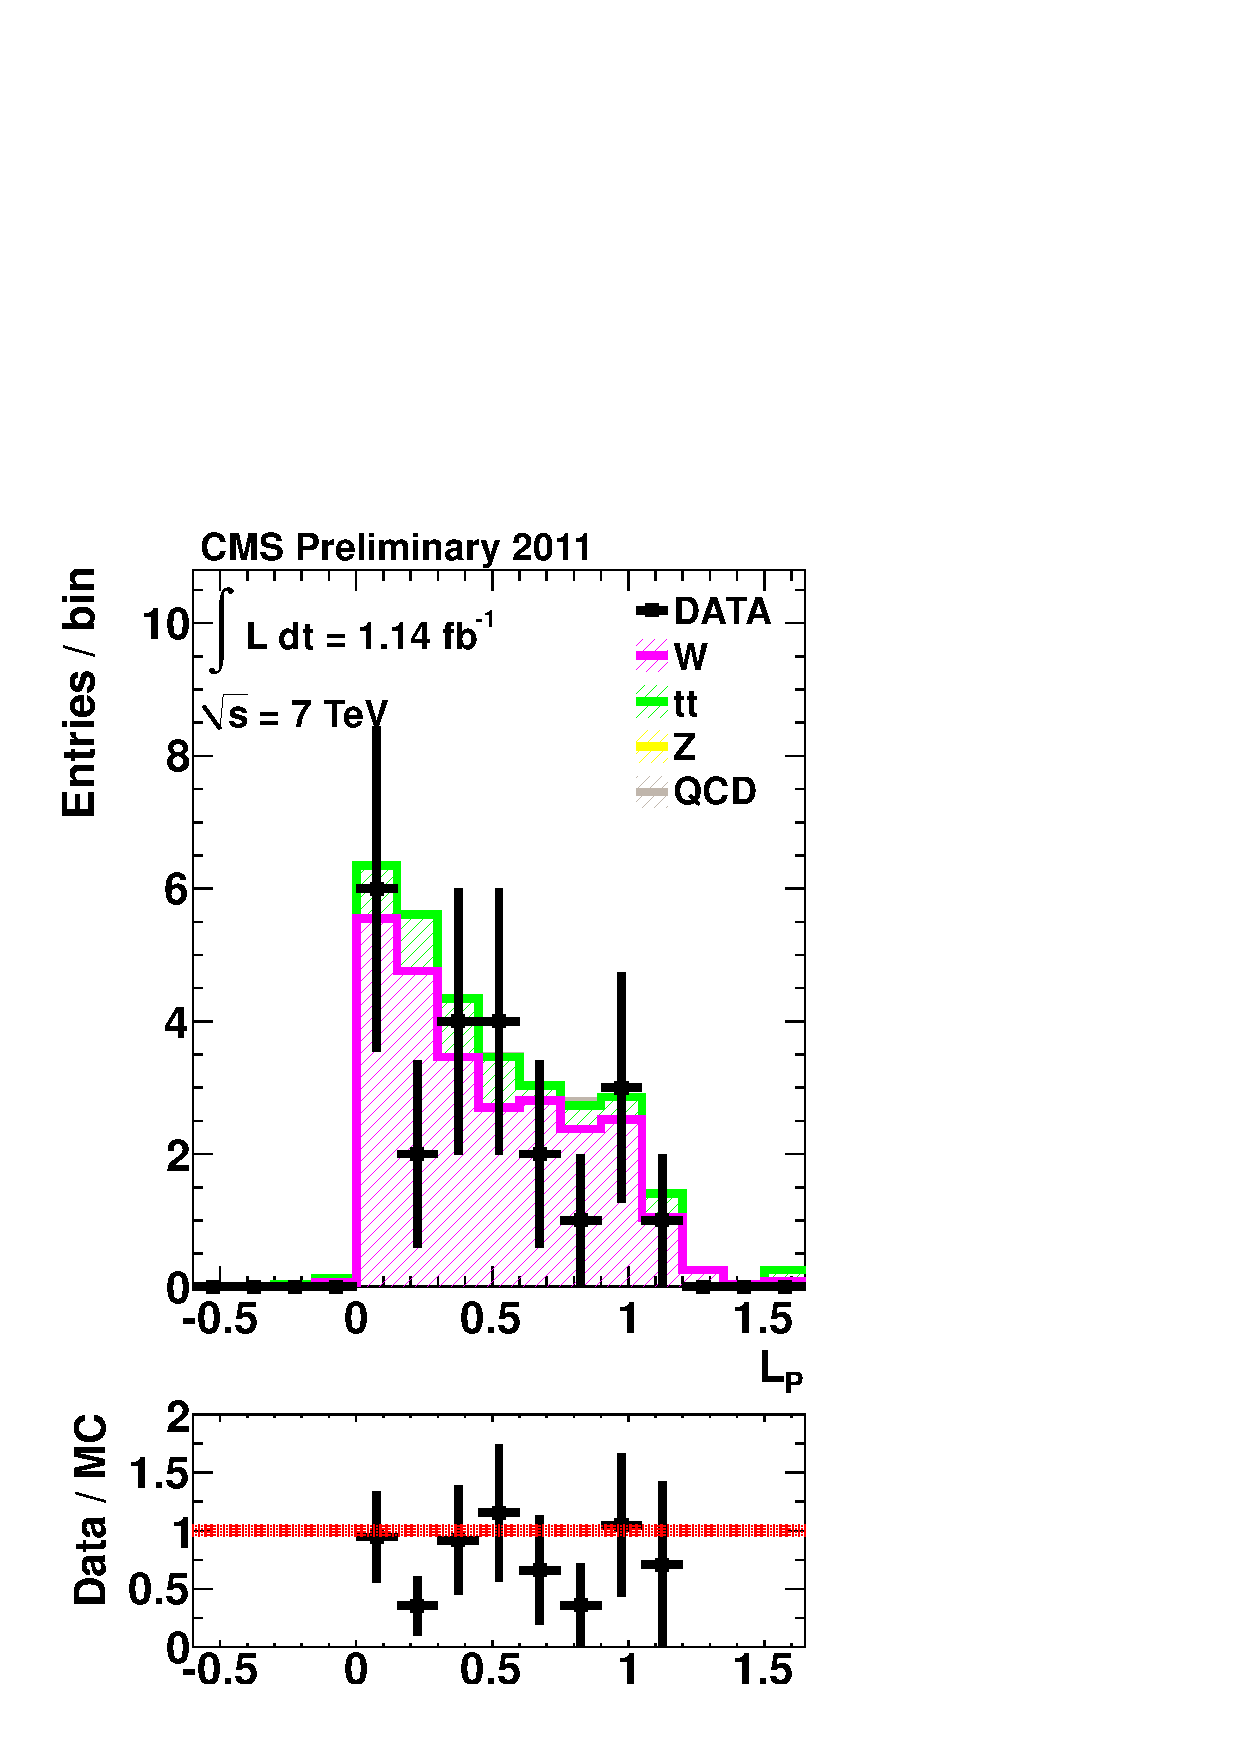
\includegraphics[width=0.3\textwidth]{fig/MuHad_LP450}}\\
\subfloat[\Pe $250 < \STlep < 350$]{\label{fig:susy_el_lp250}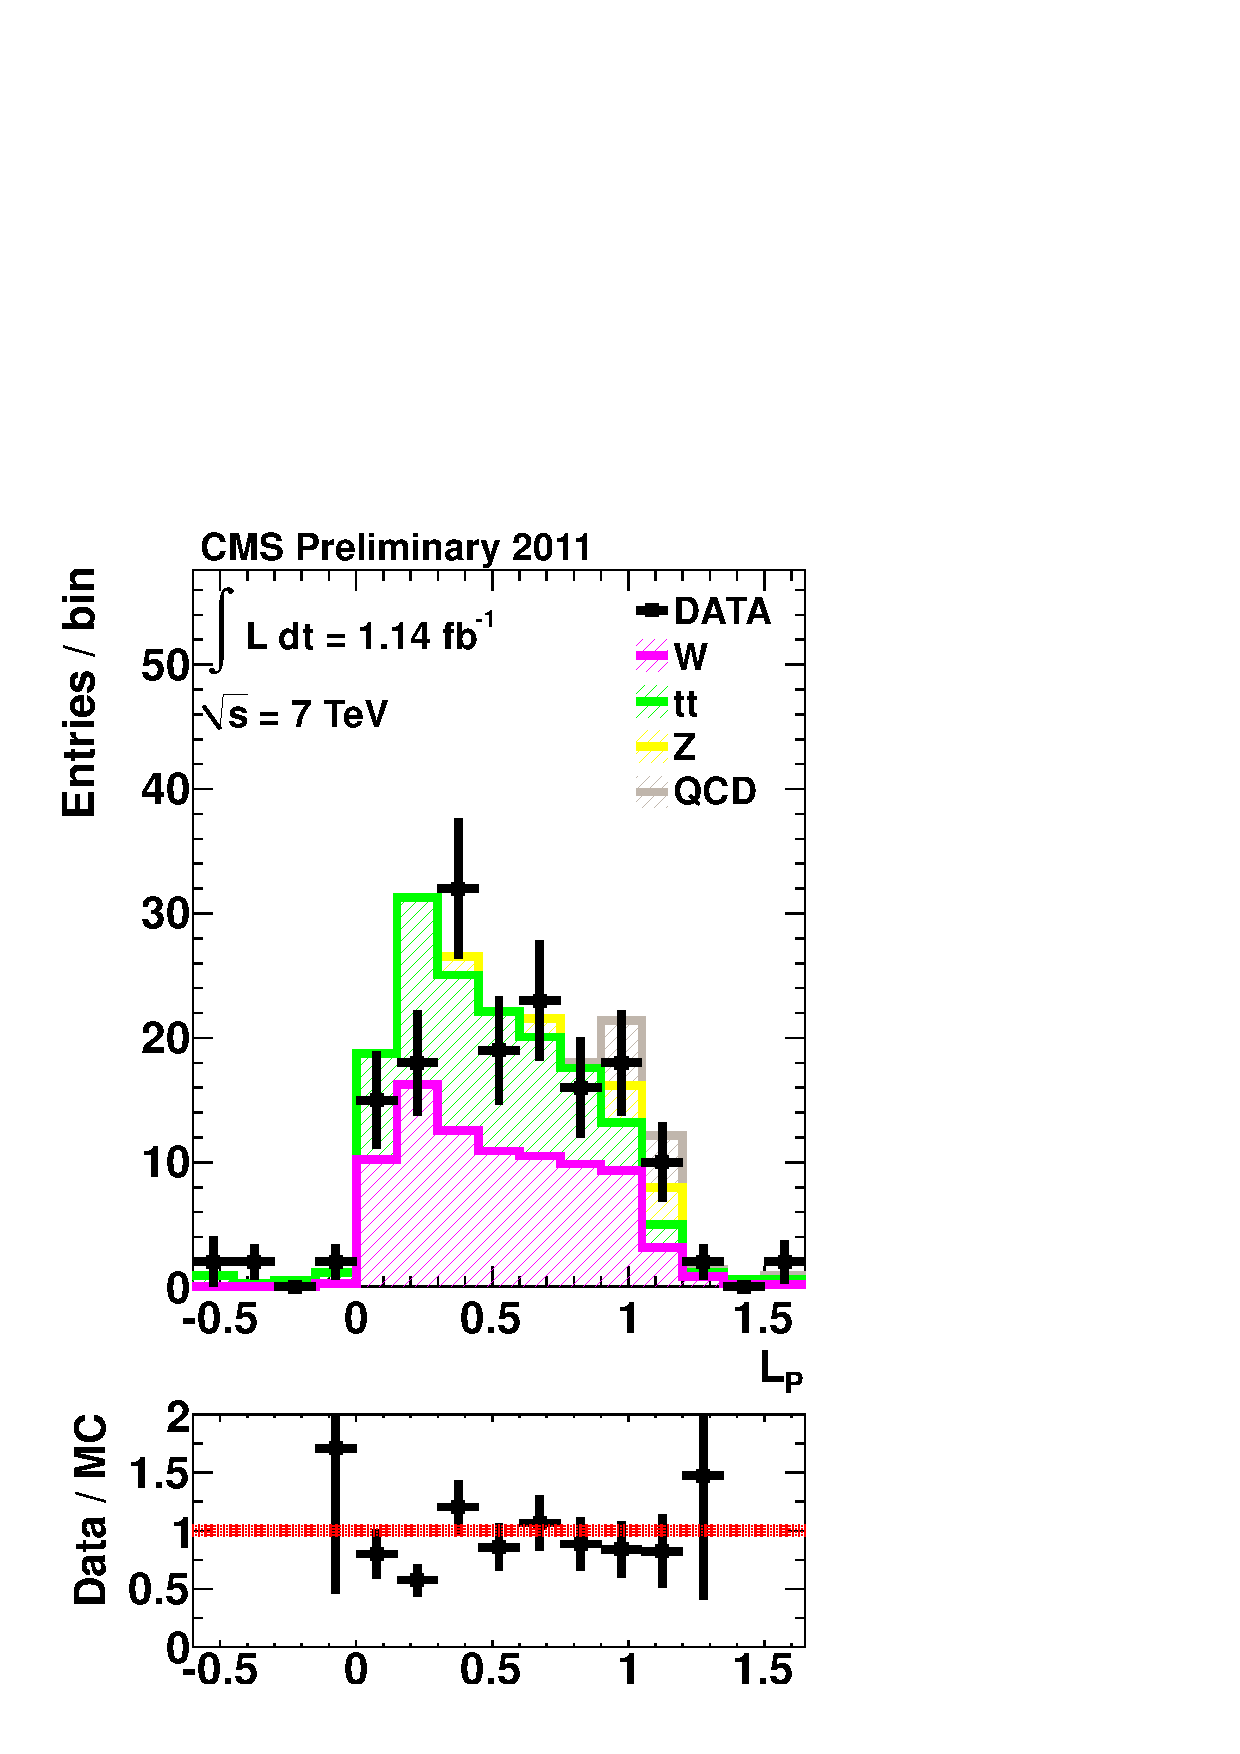
\includegraphics[width=0.3\textwidth]{fig/ElHad_LP250}}\quad
\subfloat[\Pe $350 < \STlep < 450$]{\label{fig:susy_el_lp350}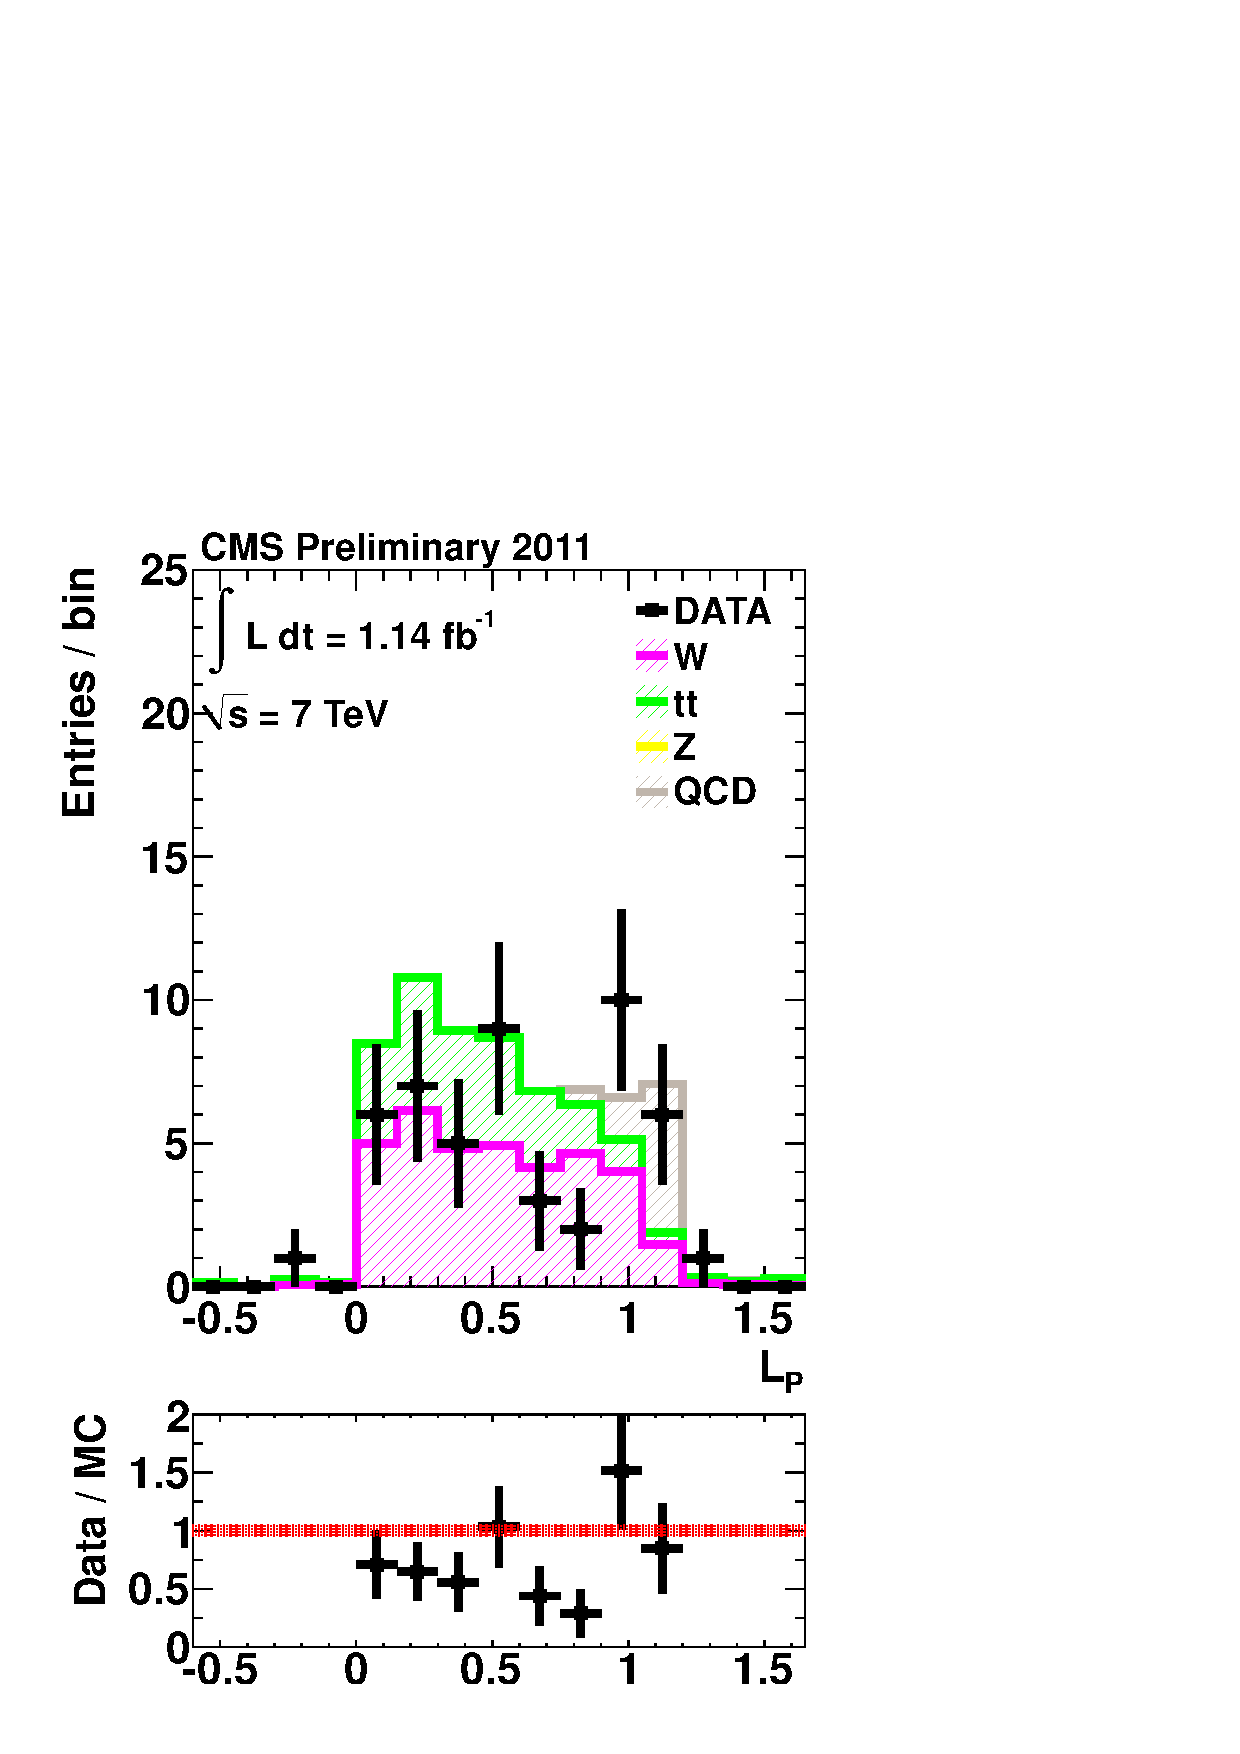
\includegraphics[width=0.3\textwidth]{fig/ElHad_LP350}}\quad
\subfloat[\Pe $\STlep > 450$]{\label{fig:susy_el_lp450}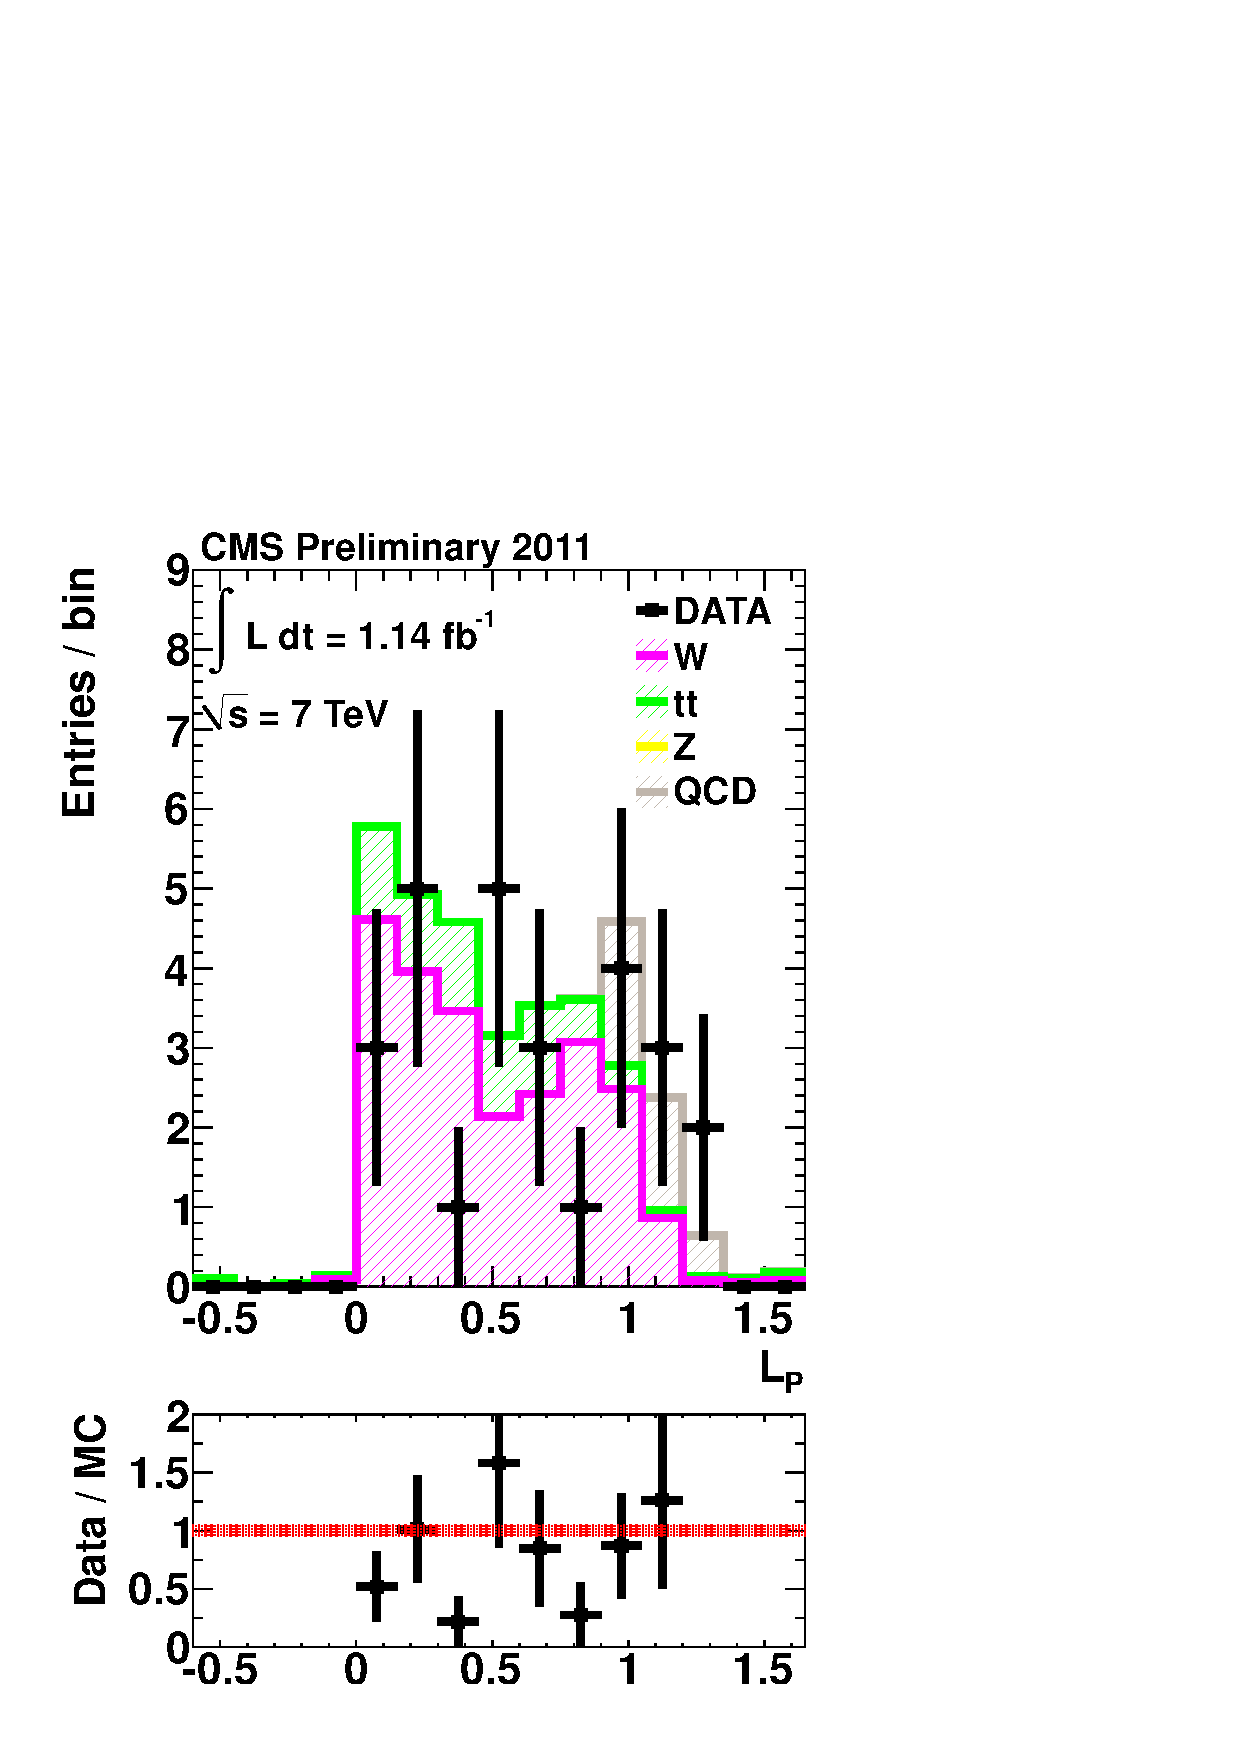
\includegraphics[width=0.3\textwidth]{fig/ElHad_LP450}}
\caption[]{Comparison of the \LP shapes in each \STlep bin between data and simulation.}
\label{fig:susy_datamc}
\end{figure}

\ctable[
cap=Event yields in data and \acs{MC} for the muon search sample,
caption=Event yields in data and \ac{MC} for the muon search sample. The column
``Total MC'' shows the expected yield from \ac{MC}. The column ``SM Estimate''
gives the result of the background prediction procedure described in the text.,
%pos=h!,
label=tbl:susy_datamc_muons,
doinside=\footnotesize
]{cccccc}{
}{\FL
                   & \multicolumn{2}{c}{Control Region (\LPcontrol)} & \multicolumn{3}{c}{Signal Region (\LPsignal)} \ML
\STlep Range (GeV) & Total MC                                        & DATA & Total MC     & SM Estimate   & DATA \ML
 $[150-250]$          & $385 \pm 7$                                       & 368  & $73.9 \pm 3.0$ & $70.6 \pm 11$   & 84 \NN
 $[250-350]$          & $116 \pm 2$                                       & 112  & $28.1 \pm 1.1$ & $27.2 \pm 4.6$  & 29 \NN
 $[350-450]$          & $43.4 \pm 2$                                     & 41   & $11.5 \pm 0.7$ & $10.9 \pm  2.3$ & 9 \NN
$>$ 450            & $18.4 \pm 0.8$                                    & 15   & $6.5 \pm 0.4$  & $5.3 \pm  1.8$  & 6 \LL
}

\ctable[
cap=Event yields in the electron search sample,
caption=Event yields in data and predictions for the numbers of \ac{EWK} and
\ac{QCD} events in the electron search sample. The sum of the \ac{EWK} and
\ac{QCD} predictions is constrained to be equal to the number of events in
data. The column ``SM Estimate'' gives the result of the background prediction
procedure described in the text. The uncertainties on these values include the full
systematic uncertainties. The uncertainties in the \ac{EWK} and \ac{QCD} columns
are only statistical.,
%pos=h!,
label=tbl:susy_datamc_electrons,
doinside=\scriptsize
]{cccccccc}{
}{\FL
                   & \multicolumn{3}{c}{Control Region (\LPcontrol)} & \multicolumn{4}{c}{Signal Region (\LPsignal)}                      \ML
\STlep Range (GeV) & QCD                                                 & EWK          & DATA & QCD         & EWK          & SM Estimate  & DATA \ML
$[150-250]$          & $39.5 \pm 15.5$                                       & $350 \pm 24$   & 390  & $1.0 \pm 0.3$ & $60.8 \pm 4.1$ & $61.8 \pm 8.7$ & 69   \NN
$[250-350]$          & $5.0 \pm 5.2$                                         & $117 \pm 12$   & 122  & 0           & $22.2 \pm 2.2$ & $22.2 \pm 4.4$ & 21   \NN
$[350-450]$          & $7.1 \pm 3.9$                                         & $28.9 \pm 6.2$ & 36   & 0           & $6.9 \pm 1.5$  & $6.9 \pm 1.7$  & 7    \NN
$>$ 450            & $6.5 \pm 5.7$                                         & $12.5 \pm 3.8$ & 19   & 0           & $4.3 \pm 1.3$  & $4.3 \pm 1.5$  & 3    \LL
}

\begin{figure}[htb]
\centering
\subfloat[]{\label{fig:susy_pred_mu}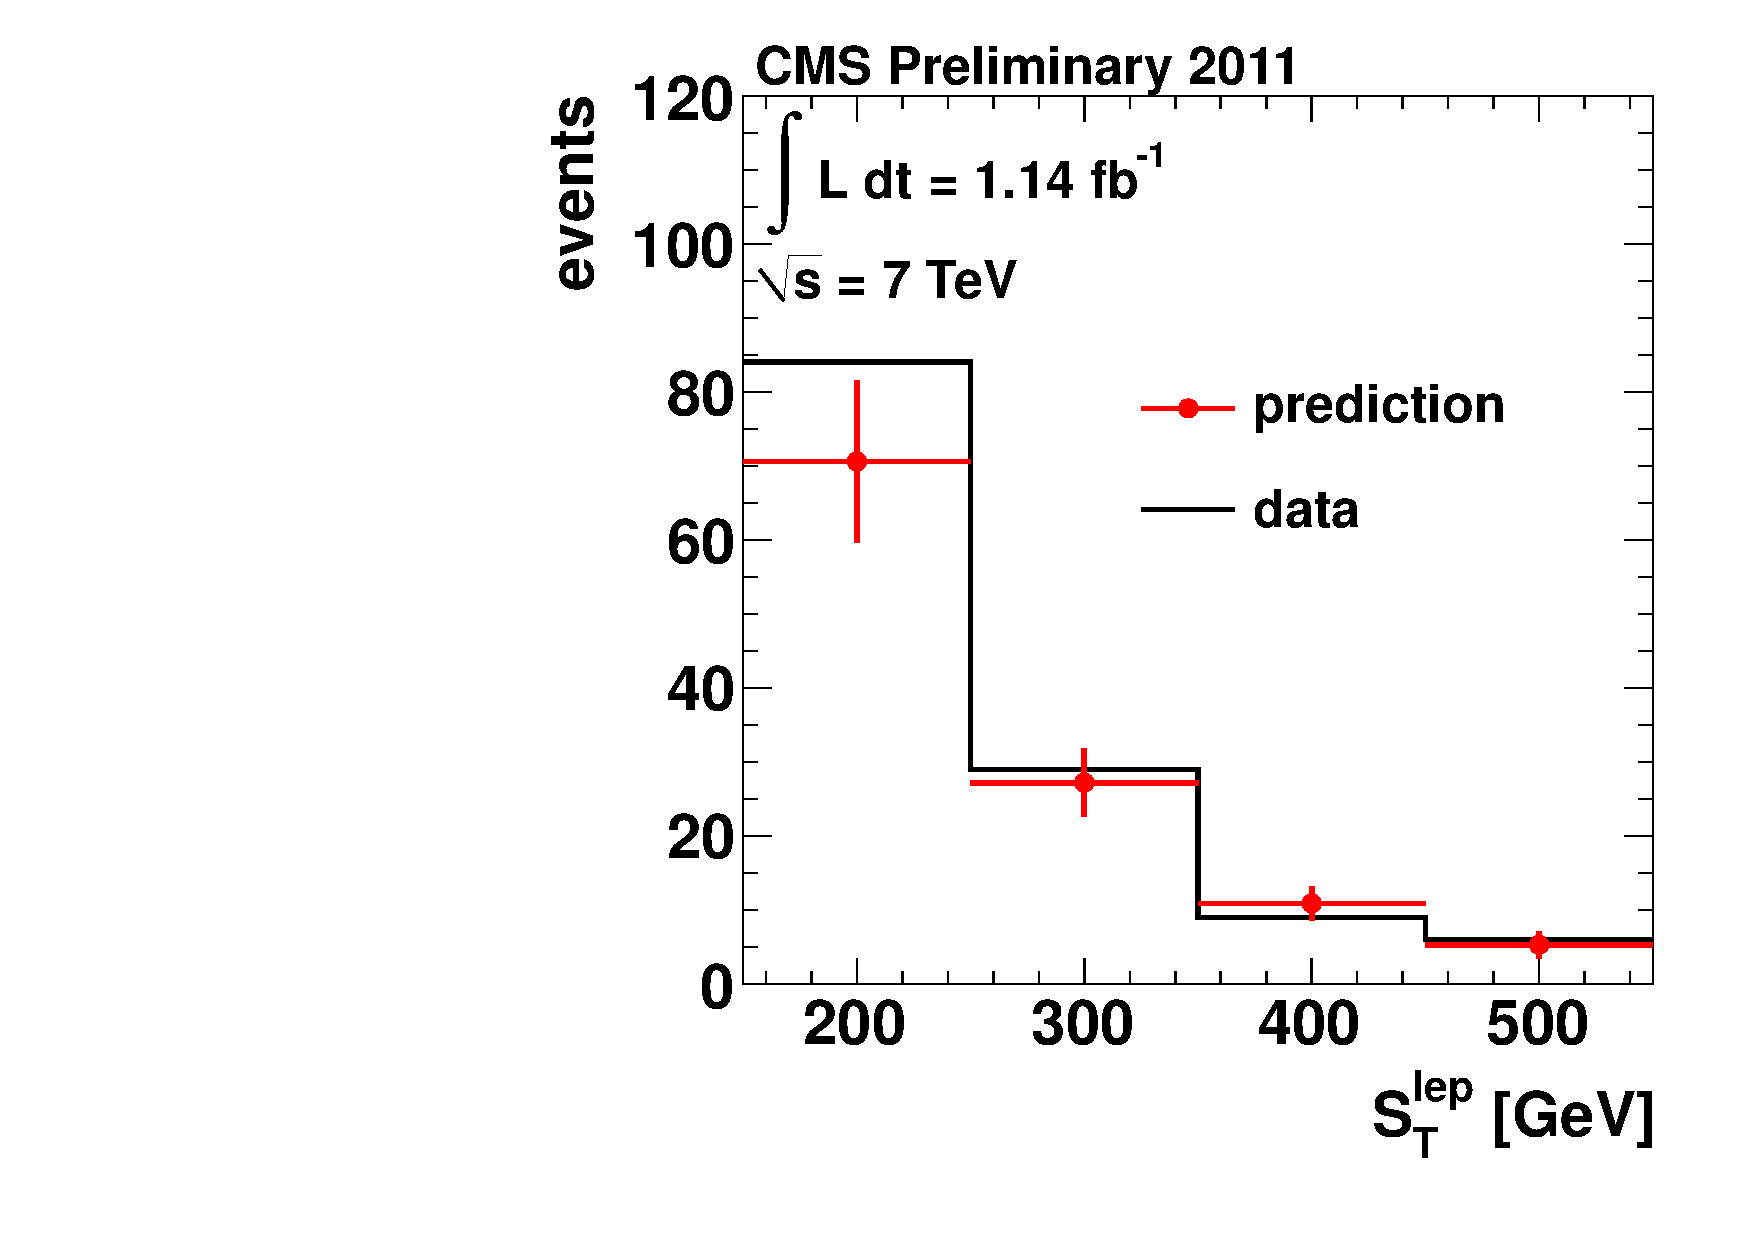
\includegraphics[width=0.4\textwidth]{fig/prediction_mu}}\quad
\subfloat[]{\label{fig:susy_pred_el}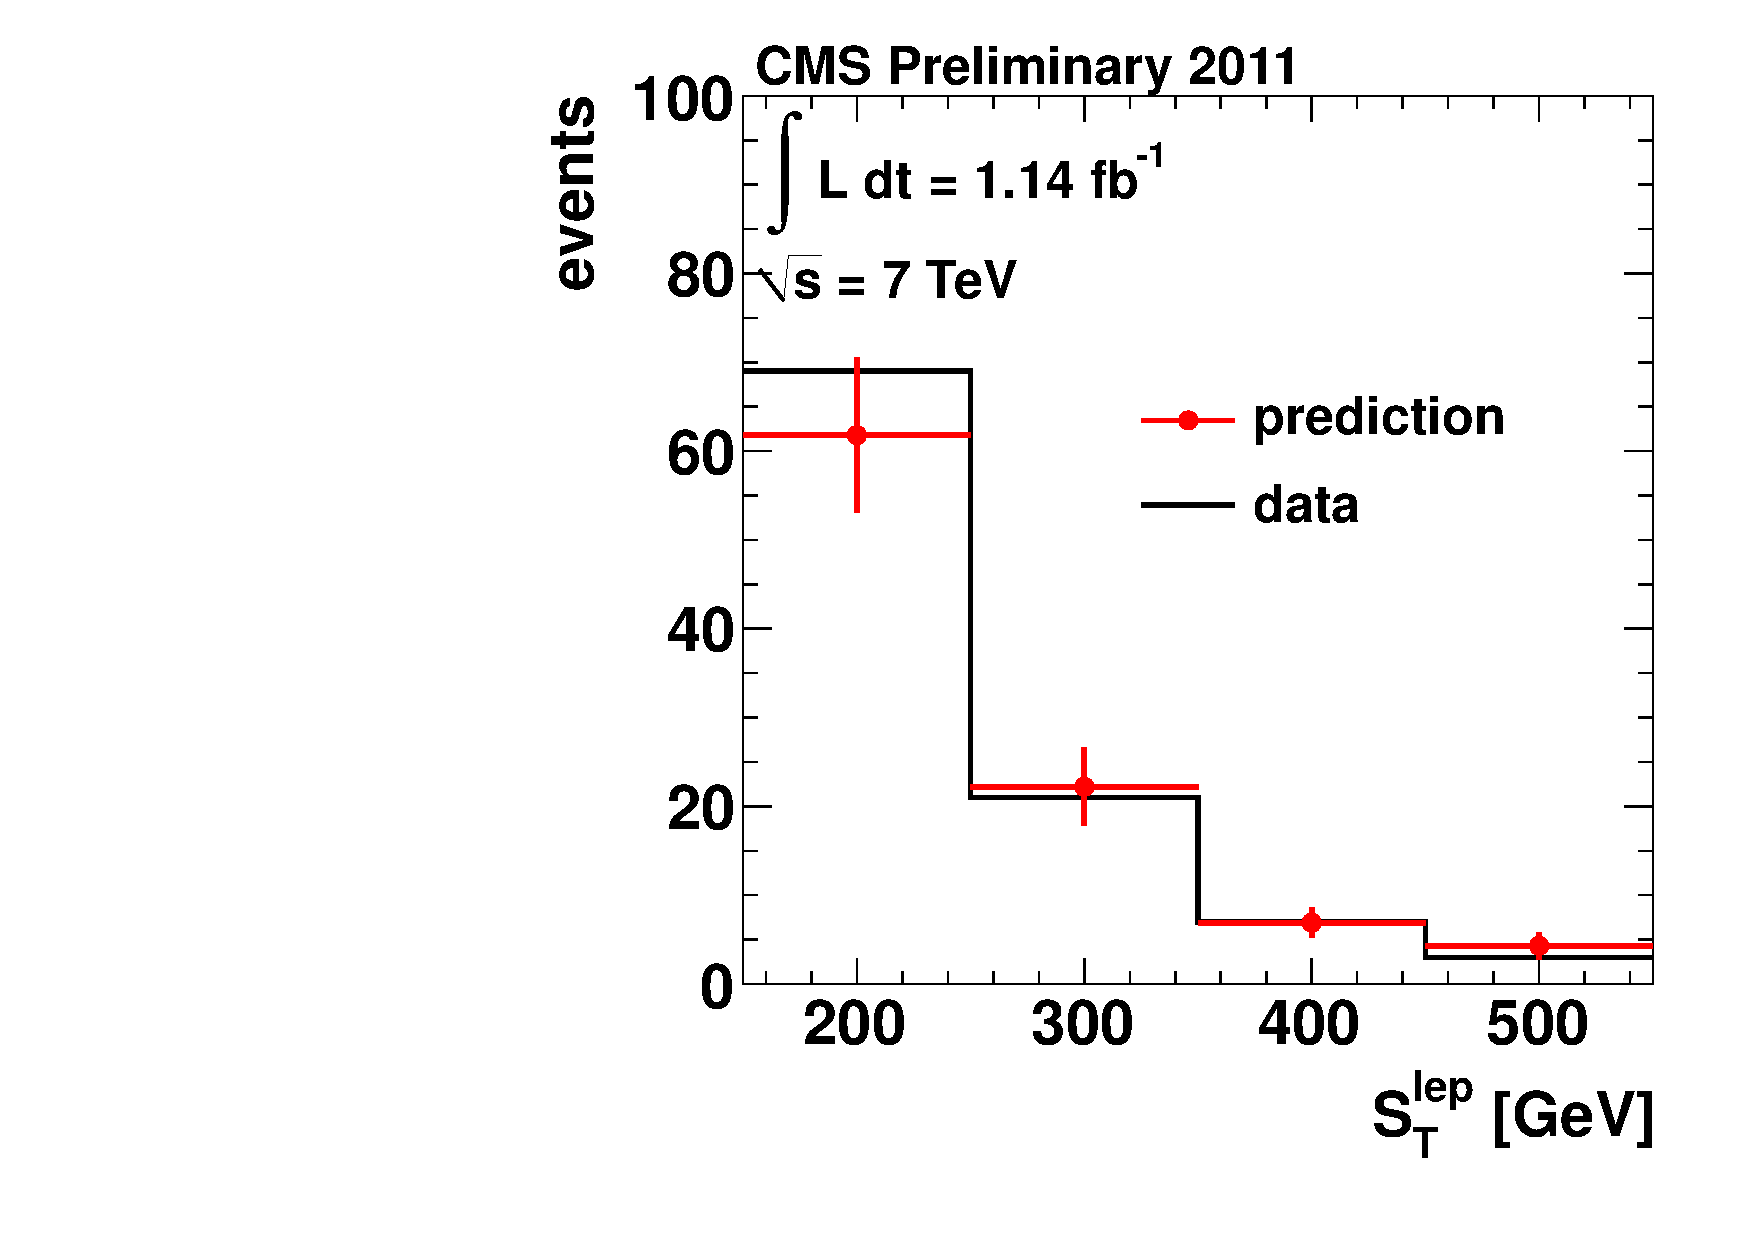
\includegraphics[width=0.4\textwidth]{fig/prediction_el}}\quad
\caption[]{Comparison of the number of events observed in the data and the
  expectations from the background estimation methods presented above, in the
  different \STlep bins.\subref{fig:susy_pred_mu} muon channel;
  \subref{fig:susy_pred_el} Electron channel.  The red error-bars indicate the
  statistical uncertainty of the data only.}
\label{fig:susy_pred}
\end{figure}